\documentclass[letterpaper, 10pt, draftclsnofoot, compsoc, onecolumn]{IEEEtran}
\usepackage{graphicx}
\usepackage{textcomp}
\usepackage{comment}

\graphicspath{ {} }

%TODO need title page from prev documents/ other packages.
% Page layout (geometry)
\setlength\voffset{-1in}
\setlength\hoffset{-1in}
\setlength\topmargin{0.5in}
\setlength\oddsidemargin{.75in}
\setlength\evensidemargin{.75in}
\setlength\textheight{8.278in}
\setlength\textwidth{6.5in}
\setlength\footskip{0.561in}
\setlength\headheight{0.5in}
\setlength\headsep{0.461in}

% Taken from Lena Herrmann at 
% http://lenaherrmann.net/2010/05/20/javascript-syntax-highlighting-in-the-latex-listings-package
\usepackage{listings}
\usepackage{color}
\definecolor{lightgray}{rgb}{.9,.9,.9}
\definecolor{darkgray}{rgb}{.4,.4,.4}
\definecolor{purple}{rgb}{0.65, 0.12, 0.82}

\lstdefinelanguage{JavaScript}{
  keywords={typeof, new, true, false, catch, function, return, null, catch, switch, var, if, in, while, do, else, case, break},
  keywordstyle=\color{blue}\bfseries,
  ndkeywords={class, export, boolean, throw, implements, import, this},
  ndkeywordstyle=\color{darkgray}\bfseries,
  identifierstyle=\color{black},
  sensitive=false,
  comment=[l]{//},
  morecomment=[s]{/*}{*/},
  commentstyle=\color{purple}\ttfamily,
  stringstyle=\color{red}\ttfamily,
  morestring=[b]',
  morestring=[b]"
}

\lstset{
   language=JavaScript,
   backgroundcolor=\color{lightgray},
   extendedchars=true,
   basicstyle=\footnotesize\ttfamily,
   showstringspaces=false,
   showspaces=false,
   numbers=left,
   numberstyle=\footnotesize,
   numbersep=9pt,
   tabsize=2,
   breaklines=true,
   showtabs=false,
   captionpos=b
}

\usepackage[latin1]{inputenc}
\usepackage[T1]{fontenc}
\usepackage[english]{babel}
\usepackage{amsmath}
\usepackage{amssymb,amsfonts,textcomp}
\usepackage{color}
\usepackage{array}
\usepackage{supertabular}
\usepackage{hhline}
\usepackage{color,soul}
%\usepackage{biblatex}
\usepackage{cite}
\usepackage{hyperref}
%\usepackage{digsig} %not a default package... just for signature field on final page.
\usepackage{url}

\usepackage{comment}

\hypersetup{pdftex, colorlinks=true, linkcolor=black, citecolor=blue, filecolor=blue, urlcolor=blue, pdftitle=SYSTEMS AND SOFTWARE REQUIREMENTS SPECIFICATION (SSRS) TEMPLATE, pdfauthor=Clinton Jeffery, pdfsubject=, pdfkeywords=}
% Outline numbering
\setcounter{secnumdepth}{4}
\renewcommand\thesection{\arabic{section}}
\renewcommand\thesubsection{\arabic{section}.\arabic{subsection}}
\renewcommand\thesubsubsection{\arabic{section}.\arabic{subsection}.\arabic{subsubsection}}
\renewcommand\theparagraph{\arabic{section}.\arabic{subsection}.\arabic{subsubsection}.\arabic{paragraph}}

\parindent0pt
\parskip 1.5ex plus 0.2ex minus 0.1ex
\makeatletter

\def\subsubsection{\@startsection{subsubsection}% name
                                 {3}% level
                                 {\z@}% indent (formerly \parindent)
                                 {1ex plus 0.1ex minus 0.1ex}% before skip
                                 {1ex}% after skip
                                 {\normalfont\normalsize}}% style

\newcommand\arraybslash{\let\\\@arraycr}
\makeatother
% Page layout (geometry)
\setlength\voffset{-1in}
\setlength\hoffset{-1in}
\setlength\topmargin{0.5in}
\setlength\oddsidemargin{.75in}
\setlength\evensidemargin{.75in}
\setlength\textheight{8.278in}
\setlength\textwidth{6.5in}
\setlength\footskip{0.561in}
\setlength\headheight{0.5in}
\setlength\headsep{0.461in}
% Footnote rule
\setlength{\skip\footins}{0.0469in}
\renewcommand\footnoterule{\vspace*{-0.0071in}\setlength\leftskip{0pt}\setlength\rightskip{0pt plus 1fil}\noindent\textcolor{black}{\rule{0.25\columnwidth}{0.0071in}}\vspace*{0.0398in}}
% Pages styles
\makeatletter
\newcommand\ps@Standard{
  \renewcommand\@oddhead{\hfill }
  \renewcommand\@evenhead{\@oddhead}
  \renewcommand\@oddfoot{\foreignlanguage{english}{\textcolor{black}{SSRS Page }}\foreignlanguage{english}{\textcolor{black}{\thepage{}}}}
  \renewcommand\@evenfoot{\@oddfoot}
  \renewcommand\thepage{\arabic{page}}
}
\newcommand\ps@FirstPage{
  \renewcommand\@oddhead{}
  \renewcommand\@evenhead{\@oddhead}
  \renewcommand\@oddfoot{}
  \renewcommand\@evenfoot{\@oddfoot}
  \renewcommand\thepage{\arabic{page}}
}

\makeatother
\pagestyle{Standard}
%\setlength\tabcolsep{1mm}
\renewcommand\arraystretch{1.3}
% footnotes configuration
\makeatletter
\renewcommand\thefootnote{\arabic{footnote}}
\makeatother
\title{Forge VR Explorer Requirements}
\author{Shawn Cross, Griffin Gonsalves, Paul Kwak}
\date{2016-11-3}


\begin{document}
\pagenumbering{gobble}
\title{Spring Progress Report}
\author{Group 20: Shawn Cross, Paul Kwak, Griffin Gonsalves}
\maketitle
\hspace*{\fill}\IEEEauthorblockA{Capstone - Spring 2017}\hspace*{\fill}
\vspace{2cm}
\begin{abstract}
This document expands upon Group 20's progress with the project as it stands as of the middle of the spring term, and includes a project summary, details of project related problems with changes and solutions, group member evaluations, and a week-by-week breakdown of the progress of the design phase. 
\end{abstract}
\IEEEpeerreviewmaketitle

\newpage
\pagenumbering{arabic}

{\centering\selectlanguage{english}\bfseries\color{black}
TABLE OF CONTENTS
\par}

\bigskip

\setcounter{tocdepth}{2}
\renewcommand\contentsname{}
\tableofcontents

\bigskip
\clearpage

\section{Introduction}
 Patti Vrobel of Autodesk of Autodesk requested our project. This project was requested to help Autodesk gain information on the experience of using Autodesk's Forge API platform as well as showcase the abilities of the Forge APIs. A a newly developed set of APIs there are many problems users may run into while attempting to utilize the APIs. Gaining feedback as well as observing the limits that can push API platform are of large importance for the evolution of the Forge platform. Our client was Patti Vrobel. \\

The Forge VR Explorer team consists of Shawn Cross, Griffin Gonsalves, and Paul Kwak. Shawn Cross was the team leader as well as in charge of implementing accessibility to files from Autodesk accounts through the use of the OAUTH and data management APIs. Additionally, implemented the ability to switch between using the local and non-local CAD files for viewing. Griffin Gonsalves was in charge of the update to the websites user interface and user experience. Paul Kwak was in charge of implementing the Data Authentication (adding the ability to log into an Autodesk account) and also setup the initial version of the Forge VR Explorer which was Vrok.it mixed with adapted code. Weekly meetings and put us in contact with Vrok.it's creator Kean Walmsley and the adapted NPM library creator Adam Nagy.

%RequirementsDocument
\newpage
\clearpage\setcounter{page}{1}\pagestyle{Standard}
\thispagestyle{FirstPage}

\bigskip

\section{Project Requirements}
{\centering\selectlanguage{english}\bfseries\color{black}
Forge VR Explorer Requirements
\par}


\bigskip

{\centering\selectlanguage{english}\bfseries\color{black}
November 4 2016
\par}
\bigskip
\bigskip
\bigskip
\bigskip
\bigskip
\bigskip
\bigskip
\bigskip
\bigskip
\bigskip
\bigskip
\bigskip
\begin{center}
	
\includegraphics[scale=0.8]{forge_logo.png}
\end{center}


\vfill
{\centering\selectlanguage{english}\bfseries\color{black}
Abstract
\par}

{\centering\selectlanguage{english}\mdseries\color{black}
	The Forge VR Explorer branches from an Autodesk prototype project called Vrok-It, which is a simple web-based 3D 
	model viewer and mobile virtual reality (VR) explorer. The project will expand upon its ability to display uploaded 3D 
	models in browser and in VR, and improve its accessibility. Conventionally, viewing 3D models in VR is a challenge if 
	you have model files on many devices, or have a headset that only works in conjunction with a smartphone. The 
	Forge VR Explorer aims to do this by utilizing a web-based software that uses the features of the Autodesk Forge API. 
	The project will also be expanded with new ideas and stretch goals as the project is developed.
\par}

\bigskip
\bigskip

\clearpage{\centering\selectlanguage{english}\bfseries\color{black}
SYSTEMS AND SOFTWARE \ REQUIREMENTS SPECIFICATION (SSRS) FOR 
\par}

\bigskip

{\centering\selectlanguage{english}\bfseries\color{black}
Forge VR Explorer
\par}

\bigskip
\bigskip
\bigskip

\begin{figure}
\centering
%\includegraphics[width=3.4362in,height=0.6134in]{SSRSTemplateA2-img1.png}
\end{figure}

\bigskip
\bigskip

{\centering\selectlanguage{english}\bfseries\color{black}
Version 2.0
\par}

{\centering\selectlanguage{english}\bfseries\color{black}
11/4/2016
\par}


\bigskip
\bigskip

{\centering\selectlanguage{english}\bfseries\color{black}
Prepared for:
\par}

{\centering\selectlanguage{english}\bfseries\color{black}
Patti Vrobel, Autodesk
\par}


\bigskip
\bigskip

{\centering\selectlanguage{english}\bfseries\color{black}
Prepared by:  
\par}

{\centering\selectlanguage{english}\bfseries\color{black}
Shawn Cross, Griffin Gonsalves, Paul Kwak
\par}

{\centering\selectlanguage{english}\bfseries\color{black}
Oregon State University
\par}

{\centering\selectlanguage{english}\bfseries\color{black}
Corvallis, OR \ 97331
\par}

\clearpage{\centering\selectlanguage{english}\bfseries\color{black}
\foreignlanguage{english}{\MakeUppercase{\ }}\foreignlanguage{english}{\MakeUppercase{Forge VR Explorer SSRS}}
\par}

\clearpage

\section{Introduction}
	The system being developed is intended to be a place in which users with CAD files can go and easily view and explore those files in both a 3D viewer and optionally in VR. The user will also be able to move through the models depending on the model that they are currently viewing. This provides a solution to those who don't have access to an expensive CAD program or VR headset as it will be a free to use web application that is usable with inexpensive VR equipment such as Google cardboard. This app is aimed at people that would want to explore a 3D model without any experience with VR or a CAD program.
 

\subsection{Scope}
	The scope of this project includes developing a new website hosting a web application.
 	This software should allow for the upload of a 3D model file to be viewed in browser as well as in a VR environment. 
	This project also aims to reduce barriers from uploading and viewing files by implementing different Forge APIs in order to improve the users 
	overall experience while using the website.

\subsection{DEFINITIONS, ACRONYMS, AND ABBREVIATIONS}
	\begin{description}
	\item{CAD} Computer Aided design is software used to design and view 3D models.

	\item{CAD file} The type of files that can be uploaded to the website for viewing in the Forge viewer. 
	We will  narrow down what types of files can be used as we progress through the development process.

	\item{FORGE}~\cite{forge2016} A collection of API services provided by Autodesk that provide 3D modeling services and tools.

	\item{Forge Viewer} This is one of the APIs in Forge. It displays 3D models from CAD files and also allows
	for user interaction.
	
	\item{Model Derivative API} This is another API in Forge. It can generate SVF files that we can utilize in the application from other model filetypes.
	
	\item{VR} Acronym for virtual reality, typically a peripheral device or smartphone
	\item{exploding model} A model viewing functionality that separates components from their original locations in order to gain an alternate view of the model.
	\end{description} 

\clearpage
	
%\subsection{REFERENCES}
\bibliography{bibfile}
\bibliographystyle{IEEETran}

\clearpage

\section{OVERALL DESCRIPTION}

\subsection{PRODUCT PERSPECTIVE}
	The product would be jump-started from the Vrok-It~\cite{Vrok-It2016} platform that has already been created. 
	We are to create a new site with some of these assets in order to provide a new experience focused on exploring a model in 3D. 

\subsection{PRODUCT FUNCTIONS}
	\begin{enumerate}
	 	\item The user is able to choose a CAD model file locally or upload one from another cloud service.
	 	
		\item Once a model is chosen or a file is uploaded the 3D models will be seen in the Forge viewer at the center of the website.
		
		\item The user will have the ability to connect a smartphone device to the website through the use of a QR scanner.

		\item Once the user has connected their a smartphone the model should be able to be viewed in VR with a the use of a VR headset such as Google Cardboard, if supported. 
		
		\item "Viewable" 3D models can be interacted with by the user in the Forge viewer in several different ways.		
		
		\item The user will be able to manipulate the model and observe in VR.
	\end{enumerate}

\subsection{USER CHARACTERISTICS}
	%perhaps easier if itemized
	When finished this product should be usable by anyone that has access to a CAD model file. If the user is wanting to use the VR 
	portion of the website then they will need access to some sort of VR headset. If the user does have access to a VR headset they 
	should not need any extra knowledge other than how to use the headset.  

\subsection{SYSTEM LEVEL (NON-FUNCTIONAL) REQUIREMENTS}

\subsubsection{Software Interfaces}
	\begin{itemize}
		\item Interface between the computer and the website, for the uploading of models from a user's local machine into the 
		website for viewing. 
	
		\item Input will be any 3D model which is sent to the model derivative api to be converted to SVF, then to the Forge Viewer where it is displayed.
	
		\item Interface between the website and the device the user wishes to view the model on. Currently vrok.it uses a QR code to accomplish this-Input is the QR code scanned by the phone, output is the manipulatable model in an environment 
	for viewing. 
	\end{itemize}
	

\subsubsection{User Interfaces}

	\begin{itemize}
		\item The main user interface will be the web application in which the user will be able to upload a  model and then view it in the Forge viewer on the  webpage. 
		\item The user will be able interact and manipulate the model inside the viewer using an interface. This interface can rotate, move, show an exploded view of the model, and more.
		\item On a smartphone, the webpage loads a compact version of the main site. 
		\item The viewer on the smartphone is fullscreen when connected, and will be manipulated the same way the webpage is currently manipulating the model.
		\item The user will be able to navigate through the model in VR using a VR headset.
	\end{itemize}

\section{SPECIFIC REQUIREMENTS}
\bigskip

\subsection{SYSTEM FEATURES}
\medskip

\subsubsection{File Uploading}

\begin{enumerate}
	\item This will allow the user to be able to upload any models that they have access to the website.

	\item
	\begin{description} 
		\item[Input] The user will select a file from their computer that they would like to upload to the website. 
		\item[Output] Finishing the upload process the model that was in the file should now be viewable on the website. 
	\end{description}

	\item
	\begin{enumerate}
		\item The user should be able to upload his/her file to the website using a standard pop-up window.
		\item The software must determine if the file is a reasonable size(<50MB), and is an accepted format. 
		\item After the file is uploaded, it is then made available to the other components of the software to be used.
		\item Users should be notified if their file was unable to be uploaded.
		\item The uploaded file should be displayed in the list of usable models on the webpage.
	\end{enumerate}
\end{enumerate}
%end of upload feature

\subsubsection{Viewable Model}

\begin{enumerate}
	\item	The user should be able to see the model that they have chosen or uploaded to the site in the Forge viewer. They 
	should also be able to interact with that model in the Forge viewer. 

	\item
	\begin{description}
		\item[Input] The user will chose from the list of predefined models or upload their own model. 
		\item[Output] The model will now be view able in the large model viewer and the user should be able to interact with that model.
	\end{description}

	\item The model must not be so large or detailed that the website can not render it.

	\item The model should be displayed in full in the Forge viewer and should not be hard to interact with. 

	\begin{enumerate}
		\item The viewer will be displayed at the center of the webpage.
		\item Once the user has selected a model for viewing or uploaded their own model, it will be displayed in the viewer. 
		\item This window must be interactive, and display the user's model correctly.
		\item The viewer should be warn the user if the model selected is too large. 
	\end{enumerate}
\end{enumerate}
%end of feature 2

\subsubsection{Smartphone Connection}

\begin{enumerate}

	\item This will enable the users to connect their phone to the Vrok-It website. This is needed so that the user will be able to view their model in a VR environment through the use of their phone and a compatible VR headset. 

	\item
	\begin{description}
		\item[Input] The user will scan a QR code located on the main page of website with a QR scanning application on their phone. 
		\item[Output] The model that is currently loaded into the Forge viewer on the website will now be displayed on the phone and ready to
		be viewed in VR. 
	\end{description}

	\item The user must have a device that is capable of using a QR scanning application. The phone also has access to an Internet 
	connection to be able to connect to the websites current session. 
	
	If the user opts to view the model in VR, then a VR headset is also required for the user's device.

	\item The phone should be connected to the website within a few seconds. This might vary depending on how good of an Internet 
	connection the user currently has. 

	\item
	\begin{enumerate}
		\item In order to provide VR functionality for an android device, the software must first establish a connection. 
		\item Using a QR scanner, the android device will be linked to a mobile version of the viewer displayed in stereoscopic format. 
		\item This requires a stable Internet connection in order to deliver the content to the device.
	\end{enumerate}
\end{enumerate}
%end feature 3

\subsubsection{Forge Authentication}
\begin{enumerate}
	\item This is used to get authentication and authorization when using Forges other APIs. This provides security for the users using 
	the APIs on the website. 

	\item The token will be created automatically every time a user accesses the website.

	\item The user must be able to gain access to the website on a laptop or desktop.

	\item 
	\begin{enumerate}
		\item During the loading of the web page the authentication API should generate a token For the user in case they want to use 
		either the data management API or the model derivative API. 
	\end{enumerate}
\end{enumerate}
%end of feature 4

\subsubsection{Data Management}

\begin{enumerate}
	\item Users that have files in A360 or in Fusion 360 should be able to gain access through those files from the
	website.

	\item
	\begin{description} 
		\item[Input] The user should be able to identify that they want to gain access to their files on either A360/Fusion360 or local. 
		\item[Output] Using the Forge Data Management API the user should then have access to the connected account's files, and to then upload a file.
	\end{description}

	\item
	\begin{itemize}
		\item The authentication API must have created a Token for the API to use.
		\item Must have an account with either A360 or Fusion 360. 
		\item Must conform to API general use cases
	\end{itemize}

	\item
	\begin{itemize}
		\item The files should load in a viewable format.
		\item The files should only be visible if they are viewable if not the user should be notified that the file
			they were trying to upload was unable to be used.
	\end{itemize}
	
	\item 
	\begin{enumerate}
		\item A place where users can enter information to gain access to their outside files. 
		\item This should be done through the use of the Forge Data Management API. 
		\item Once the user has access to these accounts they should then be able to obtain the 
		files they want to use and upload them to the Forge viewer.
	\end{enumerate}
\end{enumerate}
%End of feature 5

\subsubsection{Model Derivative}

\begin{enumerate}
	\item With the use of the Forge Model Derivative API any of the files that the user uploads will be converted into SVF files
	that are used by the model viewer
	
	\item
	\begin{description}
		\item[Input] The user will upload a CAD drawing file that they want to convert to an SVF file. 
		\item[Output] This should then return the correctly converted SVF file and it should now appear in the list of 
		viewable models on the website. If the conversion fails the user should be notified of the failure.
	\end{description}

	\item
	\begin{itemize}
		\item The authentication API must have created a Token for the model derivative API to use.
		\item The user must have used the proper CAD files to be converted. 
	\end{itemize}

	\item The program should clearly display the model in the list of viewable models.

	\item
	\begin{enumerate}
		\item The website will take the files that have been uploaded by the user and convert them to the appropriate file
		format.
		\item The website should notify the user if the file conversion has failed.
	\end{enumerate}   
\end{enumerate}
%End of feature 6

\begin{comment}
\subsubsection{Hardware Detection}

\begin{enumerate}
	\item This feature serves as a way for the software to understand the hardware its being run on. This will be the foundation for 
	giving a user feedback on potential experience viewing.

	\item
	\begin{description}
		\item[Input] The user connects their phone to Vrok-It through the use of a QR scanner. 
		\item[Output] After connection it should verify what type of device that the user has connected.
	\end{description}

	\item	Reliance on the user giving permission to allow the software to get information about hardware specifications. Similar to 
	Androids permissions the user many not want to give information out so our hardware detection may be hindered and 
	unable to function at all. 

	\item Needs to be able to obtain hardware specification as fast as possible to give users feedback immediately. The sooner 
	our software understands the user's hardware the faster it can give a recommendation about optimal viewing. 

	\begin{enumerate}
		\item The software must be able to detect the user's smartphone when it connects using the QR code provided. 
		\item When a connection is made, the software will then detect the device, verify it is supported. 
		\item If device is known, the software then will use presets for the viewer on the device, otherwise
		it should alert the user about incompatibility and performance conflicts. 
		\item These alerts will inform the user that the device will not operate optimally with the project. 
	\end{enumerate}
\end{enumerate}
%end of feature 7
\end{comment}

\subsubsection{VR device support}

\begin{enumerate}
	\item View the model currently in the viewer in a VR environment using a VR headset such as Google cardboard. The user should also
	be able move through the model in VR. This could be extended to higher end VR devices later if time permits.

	\item
	\begin{description}
		\item[Input] A functioning model uploaded to the project site and displayed in the viewer.
		\item[Output] A model displayed on the user's device that is ready to be viewed with a VR headset.
	\end{description}

	\item Depends heavily on hardware on the device that the user is using. Devices with low-end hardware will likely not be able to 
	display models that are large or have a lot of detail very well.  

	\item The models need to be able to be manipulated by the viewer. If they are too large, the models will cause errors if they are 
	modified within the viewer.  

	\begin{enumerate}
		\item The VR model viewer displayed on the Android device must be supported on Google Cardboard's lenses. 
		\item The model must be tracked properly in the model viewer. 
		\item The model displayed on the users devices should mimic any interaction that happens to the model on the webpage.
		\item The user should have the ability to navigate through the model. 
	\end{enumerate} 
\end{enumerate}
%end of feature 8

\begin{comment}
\subsubsection{Website Redesign}

\begin{enumerate}
	\item In order to accommodate for new features, we would like to redesign the landing, and key interaction areas of the website using the html, css and javascript project as started with the Vrok-it project. Ideally, this will increase the site's usability by decreasing the amount of time used to interact with the website and making the site look more cohesive and presentable.
	\item This website must support the Forge API, the Forge viewer, and must be viewable on a smartphone browser. 
	\item The website must be able to properly load and display the project assets like the Forge Viewer. 
	\item The updated site will include a new main page for the project, as well as being able to expand the site as necessary.
	\item Key functionality such as uploading a model file and viewing the file should be clearly visible to the user.
		
\end{enumerate}
%end of feature 9
\end{comment}

\clearpage
\section[GANTT CHART]{\selectlanguage{english}\rmfamily\bfseries\color{black}
GANTT CHART}

\begin{center}
	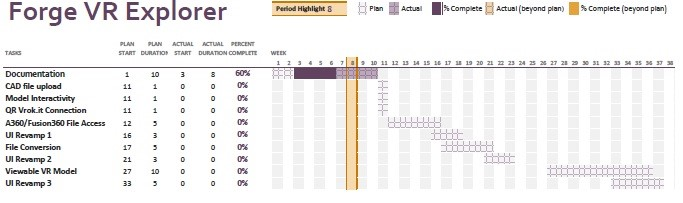
\includegraphics[scale=0.8]{GanttChart.jpg}
\end{center}
\clearpage
\section[UPDATED GANTT CHART]{\selectlanguage{english}\rmfamily\bfseries\color{black}
UPDATED GANTT CHART}

\begin{center}
	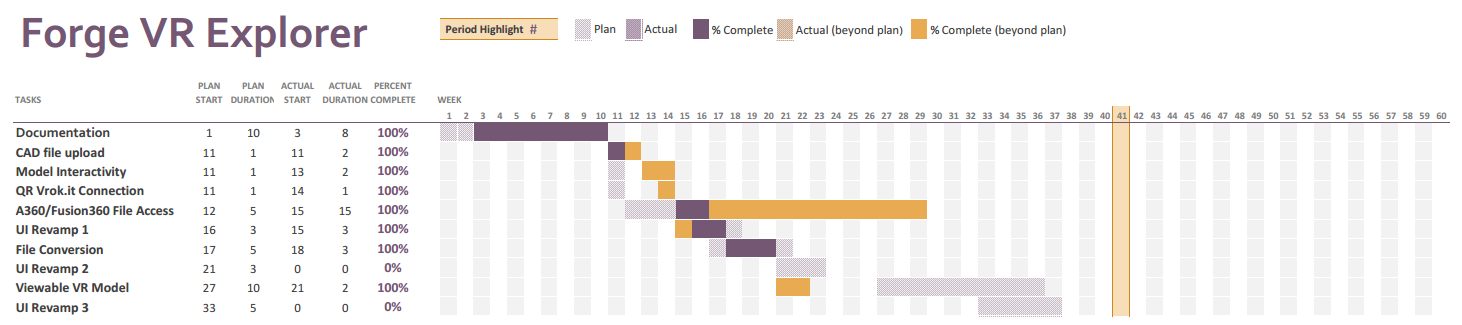
\includegraphics[scale=0.8]{NewGantt.png}
\end{center}


%DesignDocument
\newpage
\section{Design Document}
%\clearpage\setcounter{page}{1}\pagestyle{Standard}
\thispagestyle{FirstPage}

\bigskip

{\centering\selectlanguage{english}\bfseries\color{black}
Forge VR Explorer Design Document
\par}

\bigskip

{\centering\selectlanguage{english}\bfseries\color{black}
December 2 2016
\par}
\bigskip
\bigskip
\bigskip
\bigskip
\bigskip
\bigskip
\bigskip
\bigskip
\bigskip
\bigskip
\bigskip
\bigskip
%\begin{center}
%	
\includegraphics[scale=0.8]{forge_logo.png}
%\end{center}

\vfill
{\centering\selectlanguage{english}\bfseries\color{black}
Abstract
\par}

{\centering\selectlanguage{english}\mdseries\color{black}
	The Forge VR Explorer branches from an Autodesk prototype project called Vrok-It, which is a simple web-based 3D 
	model viewer and mobile virtual reality (VR) explorer. The project will expand upon its ability to display uploaded 3D 
	models in browser and in VR, and improve its accessibility. Conventionally, viewing 3D models in VR is a challenge if 
	you have model files on many devices, or have a headset that only works in conjunction with a smart-phone. The 
	Forge VR Explorer aims to do this by utilizing a web-based software that uses the features of the Autodesk Forge API. 
	The project will also be expanded with new ideas and stretch goals as the project is developed.
\par}
\clearpage

\section{Introduction}
The Forge Explorer is a web application capable of accomplishing several tasks. The web app allows for the upload of CAD files, renders them on the website utilizing the Forge APIs, allows the transfer and rendering of the models onto a user's mobile device, and then has the capability to allow the user to view the models using Google Cardboard or similar VR headsets- all in one place. This document aims to delve into the design of several key pieces of functionality and seeks to expand their design and structure. This spans from the overarching web layout, to individual components the Forge API the team will be implementing into the project.
\subsection{Scope}
The scope of this document covers the information regarding user experience data flows, the software design description and the design structure of the software. This design document includes information critical to the development of the project as a whole. This document does not cover specific implementation decisions or quality requirements.
\subsection{Purpose}
The purpose of this software design document is to describe the user experience flows and provide the software design description to its intended audience. Additionally, this document provides a framework for the project that the developers will be using in order to assess the progression of the software through its development lifespan. This includes the detailed description of critical design entities, components, and systems working together in the project.
\subsection{Intended audience}
This document is targeted at developers building and implementing the software, and the stakeholders who include: Patti Vrobel, the Autodesk Forge API team,  and developers of the original "Vrok-it" project that this is based off of. Core stakeholders also are working with the project group in order to maximize the projects potential.

\subsection{Influences on SDD preparation}
The SRS is the main influence on the SDD as it holds the requirements and features determined necessary by all the stakeholders. This drives the design to meet those requirements to properly satisfy all stakeholders. However, this also means that it sets the design constraints.

\subsection{Design verification and design role validation}
In order to verify that our software meets requirements, test cases will be used in order to walkthrough the system and demonstrate the actual functionality of the software system. In terms of user experience the verification and validation will be mainly done through some primary tests with Autodesk with final okay coming from the clients.

\subsection{Design stakeholders and their concerns}
	The primary stakeholder for this project is Patti Vrobel who works for Autodesk. User experience is a primary focus of both Patti and Autodesk, and serves as an overarching goal for the project. The project addresses this by adding and altering features to make the website more accessible for users.

%\bibliography{bibfile}
%\bibliographystyle{IEEETran}

\section{Definitions}
\begin{description}
	\item{CAD} Computer Aided design is software used to design and view 3D models.

	\item{CAD file} The type of files that can be uploaded to the website for viewing in the Forge viewer. 
	We will  narrow down what types of files can be used as we progress through the development process.

	\item{FORGE}~\cite{forge2016} A collection of API services provided by Autodesk that provide 3D modeling services and tools.

	\item{Forge Viewer} This is one of the APIs in Forge. It displays 3D models from CAD files and allows for interaction with the model through clickable controls.
	
	\item{Model Derivative API} This is another API in Forge. It can generate SVF files that we can utilize in the application from other model filetypes.
	
	\item{VR} Acronym for virtual reality, typically a peripheral device or smartphone

	\item{exploding model} A model viewing functionality that separates components from their original locations in order to gain an alternate view of the model.

	\item{SVF file} The file format used by the forge viewer
	
	\item{SDD} Software Design Description, the document detailing the design of the systems for the project.
	
\end{description} 

\section{Design Views}
\subsection{Website Interface}
Because the website is the focus of the project, we are hosting a new version of the website on a new project domain. The primary requirements for the website are to properly host, arrange and display all of the individual components of the project cohesively. This includes the components of file uploading, authentication, the forge viewer, and mobile device connection software. The main webpage serves as the central interface for the project, which is critical to the user experience. This planning is necessary in order to have control over the project hosting, and to test and deploy updates that will help make the application easier to use and faster to deploy.

The interface will assist in the development phase by shortening the amount of time needed to implement initial setup to the website, which also increases the ability to spend time on other features of the project. This interface does not focus on the technical aspects of the components, and serves to ensure that the project heads toward a positive user experience though its simplicity and useful features. Technical details have been omitted as necessary to the diagram to emphasize some of the larger structure of the project as a whole. 

\subsection{Interface Viewpoint: Interface}
\begin{itemize}
	 \item[]\textbf{Forge Viewer} Implementing the Forge Viewer into the page will involve calling the API from a script embedded in the page. The individual required files for the viewer are held in the site source files.
	
	\item[]\textbf{Forge Viewer Navigation} This component of the project encompasses the control modifications and adjustments made to the viewer to allow model exploring.
	 
	\item[]\textbf{File Upload} The file upload functionality will be available on the main page in a specific area. This would include 
	
	\item[]\textbf{Smartphone QR Code}  The smartphone QR code will also have its own page section and will be viewable on the main page of the site.
	
	\item[]\textbf{Model Derivative} This component is essential in preparing the model to be used in the viewer. It is used as a method of transforming a given model of one of many supported formats to SVF. This is accomplished by using an API call to the Model Derivative API.
	
	\item[]\textbf{Information and Other Site Content} The website will eventually come to encompass more content as the project progresses in development. These changes will be noted in blogs, and will be made visible on the project website. These additions to the site will most likely come as feature updates to previously described components or new features on new pages of the site.	
\end{itemize}

\subsubsection{Design relationships}
The main webpage represents the core of the project, bringing in each component referenced in the document. Each component is loaded in either  by their respective API calls or plugins embedded in the page.
\begin{figure}[ht]
	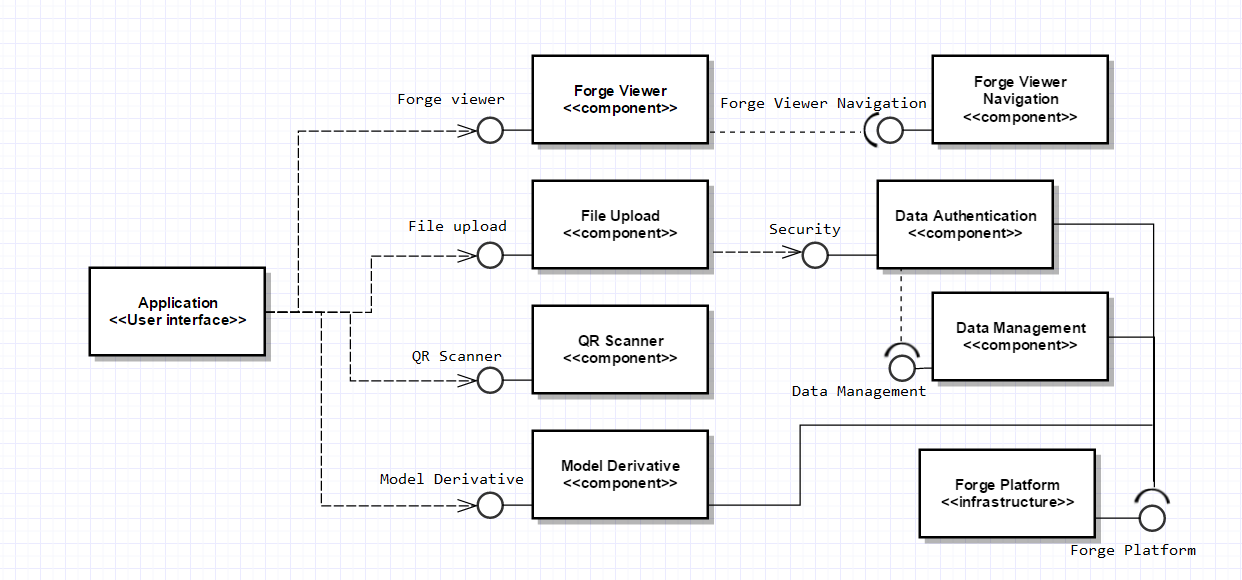
\includegraphics[scale=0.30]{WebInterface.png}
	\caption{Interface UML 2 component diagram}
\end{figure}

\subsection{Model Viewer}
\label{modelView}
The Forge Viewer is what powers the Explorer's 3D model viewer. By our requirements, the user must be able to see and interact the model they uploaded from the CAD file. This is accomplished by using the Forge Large Model Viewer, which uses WebGL rendering to display a SVF model in a specified area of a webpage. The model must be able to be manipulated and explored with both simple and intuitive controls. This includes both a viewer on a desktop machine as well as a separate viewer that is exclusively displayed on the smartphone. The user interacts with the model using the controls displayed on top of the viewer, which then modifies the camera in the actual viewer and in turn modifies the camera for the mobile device if connected. If a keyboard is connected, the inputs will be sent to the viewer for movement control.

\subsection{Interface Viewpoint: Interaction}
\begin{itemize}
	\item[]\textbf{Main Viewer Window} By default, there will be at least one viewer within the desktop website after a completed their file upload.  This includes the Viewer Controls component. The viewer uses a WebGL graphics backend that is integrated into the webpage, then called with the Forge API. If an error is detected, the viewer should fall back to an inactive state.

	\item[]\textbf{Listed Models} When a user first visits the website there will be a default list of various models that they will be able to select and view in the model. Once selected the model will be loaded into the viewer and become available for the user interact with. The user will also be given an option to upload their own models to view and interact with as well. 
	
	\item[]\textbf{Viewer Controls} The viewer is interacted with by using the Large Model Viewer's API, which is a small set of controls in a compact interface that appears at the bottom of the viewer. This set of controls can rotate, zoom, explode, or toggle settings for viewing the model. If a keyboard is connected, then a set of keys can be used to control the viewer in a basic and straightforward manner.
	
	\item[]\textbf{Model Viewer Navigation} This allows for keyboard and mouse input as a new option for controlling the Forge Viewer. This will essentially enable the model viewer to explore the 3D space around the model, and will be enabled within the API.

	\item[]\textbf{Mobile Viewer} The Main Viewer must control a separate instance of the Viewer that runs exclusively for the connected smartphone, and matches the exact position and viewing of the desktop viewer. The main viewer is also responsible for handling the controls for the second viewer. These viewers are hosted within the web page.
	

\end{itemize}
\subsubsection{Design Relationships}
	The uploaded file will be sent to the Viewer from the model derivative API described in section \ref{model derivative} after the file type is verified.
	
	The viewer is present on the smartphone and the web page. 

\subsubsection{Design Constraints} the Viewer requires the proper SVF Format in order to display a model. 
\begin{figure}[ht]
	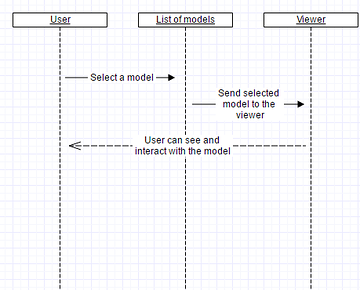
\includegraphics[scale=0.65]{viewerfromlist_360.png}
	\caption{Forge Viewer List View Interface}
\end{figure}

\begin{figure}[ht]
	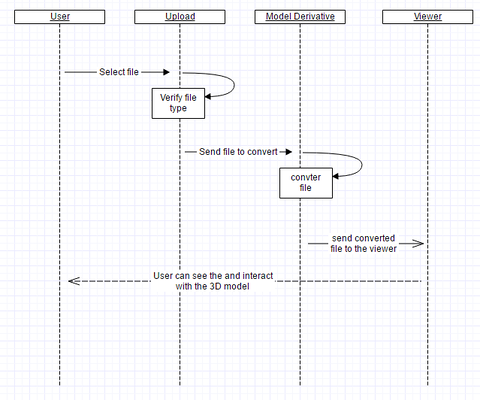
\includegraphics[scale=0.80]{viewerwithupload_480.png}
	\caption{Model Viewer Upload Option}
\end{figure}





\subsection{Local file upload}
\label{local}
	The user should be able to upload their own CAD files from a local storage device that they have access to. This will be some sort of button that is easily identifiable by the user that once selected will allow the user to browse through the local files on the current machine and select the CAD file that they would like to view. Once the file is selected the website should verify that the file is an allowed CAD drawing file. If the file is of the correct file type then the file should be converted to the SVF file type that is used by the forge viewer API. The user should be notified that the file was successfully uploaded to the website and the model that was in the file should be displayed in the list of choose-able models as well as displayed in the viewer. 

\subsection{Interface viewpoint for local file upload}
\begin{itemize}
	\item[]\textbf{local upload button} There will be a button on the website for uploading files from local storage on the users machine. This button should be easy for the user to identify. Once the user has pressed the button then the user should have access to the local files on their machine.
	\item[]\textbf{file selection} The user should be able to then navigate through their local files to find the CAD file that they are wanting to view.
	\item[]\textbf{file type verification} Once a file has been selected by the user the website should verify that the file is actually usable. This should be done by checking that if the file is a CAD drawing file type that can be converted into an SVF file that is used by the viewer. If the file is a usable file then the website 			should simply proceed and convert the file. If the file is not the correct file type then the user should be notified of this and prompted to select a different file.  
	\item[]\textbf{file size verification} Large file may not work well in the viewer in this case the website should determine if a file is to large for the viewer to handle. If the file the user has selected is to large then the user should be notified that the selected file is to large and be prompted to select a different file.
	This can be done at the same time as verifying the file size.
	\item[]\textbf{file conversion} The file conversion will be done through the use of the forge model derivative API described in. If the conversion request was successful then the file should be added to the current list of viewable models and also placed in the viewer. If the conversion request is unsuccessful then the user should be notified that their file could not be converted. 
\end{itemize}

\subsubsection{Design relationships}
	The uploaded file will be sent to the model derivative described in section \ref{model derivative} after the file type is verified.
	
	The converted file will be sent to the viewer described in section \ref{modelView}. 

\subsubsection{design constraints} require that the user has the file that they are wanting to use on the current machine that they are using. They will also only be able use CAD drawing file when uploading a file to the website.  


\subsubsection{Design rationale}
	The reason for only letting users only use the CAD drawing file types because the files need to be converted to an SVF file to be used in the viewer. The conversion to SVF files is done using the model derivative API, and this API can only convert files that are CAD drawing files. 

\begin{figure}[ht]
	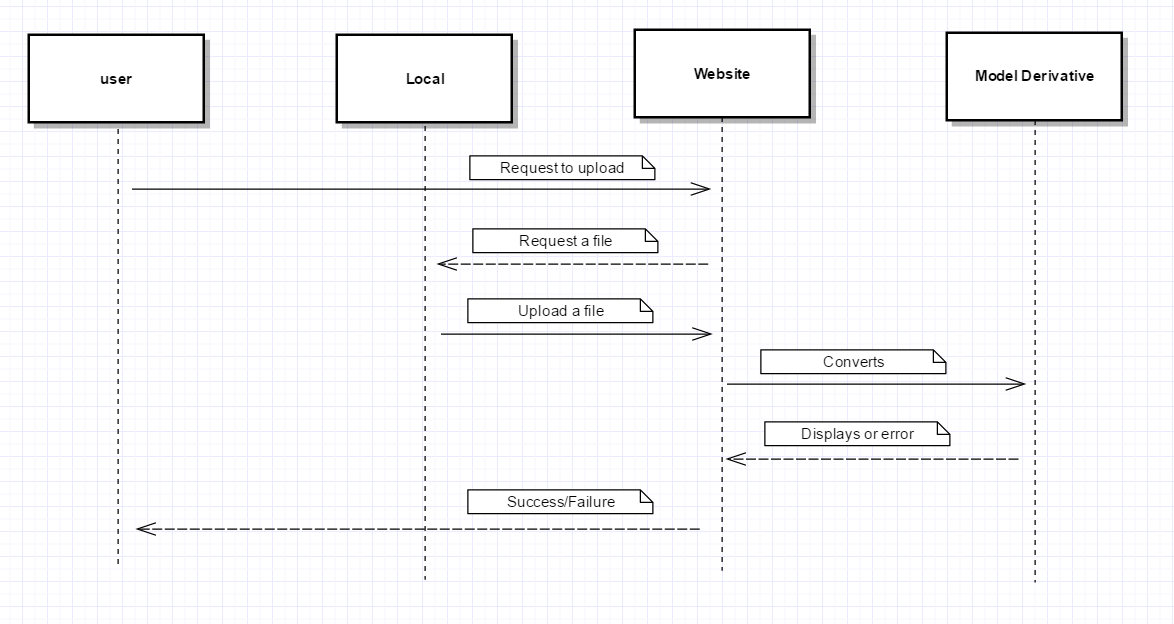
\includegraphics[scale=0.45]{localUpload.png}
	\caption{local file upload UML}
\end{figure}

\subsection{Non-local file upload}
\label{nonLocal}
	The user should be able to  access their files that are on an outside storage device and then upload these files to the website. There should be a button that the user can use to login to there outside storage. Once logged in there should be an interface that the user should be able use to navigate to the file that they want. After they have navigated to the file they want they should be able to select it and have it be uploaded to the viewer.  Our website should verify that the selected file is of the correct file type and size as well as convert the file to an SVF file using the model derivative API. If for any reason there is a failure in the file uploading process then the user should be notified of that failure and informed how to proceed.

\subsection{Interface viewpoint for non-local file upload}
\begin{itemize}
	\item[]\textbf{non-local interface} This interface should be easy for the user to understand and navigate. They should be able to quickly and easily find any of the files that they are looking for.
	\item[]\textbf{user login} Using the data management API the user will be asked to login to there Autodesk account to receive an authentication token. Once logged in the user will have access to any files located in their Autodesk storage systems. 
	\item[]\textbf{file type verification} Once a file has been sent to the website from the outside storage, it should verify that the file is compatible with the types of files used by the model derivative API. This should be done by checking that if the file is one of the 60 different file types that can be converted into an SVF file. If the file is a usable file then the website should simply proceed with converting the file. If the file is not the correct file type then the user should be notified there was a problem and prompted to select a different file.  
	\item[]\textbf{file selection} After the user has access they should then be able to navigate to the correct storage system their file is in and gain access to their files. Once a file is selected it should then be returned to the website. If returning the file is unsuccessful then the user should be notified and prompted to try 
	again.
	\item[]\textbf{file size verification} Large file may not work well in the viewer, in this case the website should determine if a file is to large for the viewer to handle. If the file is over 2MB then they should be warned that this might result in some the viewer not working at top performance. If the user has selected a file larger than 15MB then the user should be notified that this file is to large to handle and be prompted to select a different file.
	\item[]\textbf{file conversion} The file conversion will be done through the use of the forge model derivative API. If the conversion request was successful then the file should be added to the current list of viewable models and also placed in the viewer described in section \ref{modelView}. If the conversion request is unsuccessful then the user should be notified that their file could not be converted. 
\end{itemize}

\subsubsection{Design relationships}
\begin{itemize}
	\item[]\textbf{Authentication and file upload} the user will receive a token from the OAuth API that will allow them to access the data management and model derivative APIs \ref{Three legged}
	\item[]\textbf{Data management API and file upload} the user will gain access to there files through the use of the data management API described in section \ref{A360}
	\item\textbf{Model derivative and file upload} the uploaded file will be sent to the model derivative described in section \ref{model derivative} after the file type is verified.
	\item[]\textbf{Viewer and file upload} the converted file will be sent to the viewer described in section \ref{modelView}. 
  \end{itemize}

\subsubsection{design constraints} 
	require that the file or file that the user is wanting to upload be located in the outside storage that they are wanting to use. They will also only be able use CAD drawing file when uploading a file to the website.  

\subsubsection{Design rationale}
	The reasoning letting users only use the CAD drawing file types is that the files will need to be converted into an SVF file that is usable by the forge viewer. The conversion to SVF files is done using the model derivative API, and this API can only convert files that are CAD drawing files. This will also keep the list of models that a user can select from being populated with files that don't do anything because they don't work in the viewer.  

\begin{figure}[ht]
	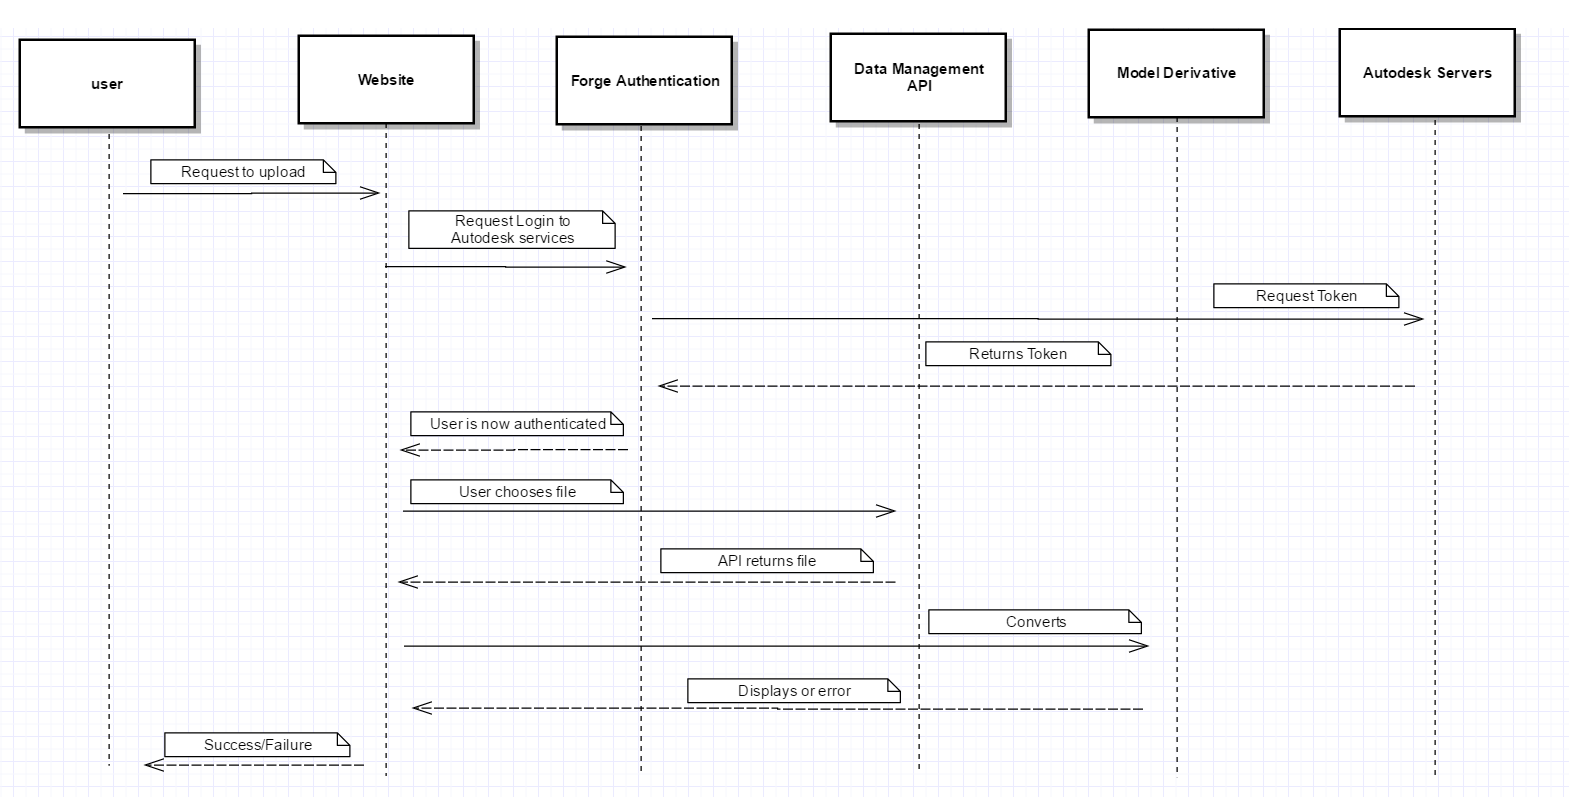
\includegraphics[scale=0.35]{nonLocalUpload.png}
	\caption{non-local file upload UML}
\end{figure}

\subsection{Mobile device connection}
\label{mobileDevice}
	The user should be able to connect their mobile device to the websites current session through the use of a QR code on the web page. The user will need to have a some way to scan the QR code with their mobile device. Once connected to the device the user should be able to see what is in the viewer on their device.

\subsection{Mobile device connection Interface viewpoint}
\begin{description}
	\item[]\textbf{QR code} There should be a QR code generated at the beginning of every session on the web page. This will be done through the use of a JQuery plug-in~\cite{QR2016} that generates QR codes. The QR code should be somewhere on the web page that is easy for the user to find. 
	\item[]\textbf{QR scanner} The user will need to have a way to scan the QR code. This will most likely be done through the use of an application on the users phone that will use there camera to scan the QR code. Any application that the user gets to scan the code should all work with the QR code on the website so there is no need to suggest a specific QR scanner to the user. 
	\item[]\textbf{device connection} Once the user has successfully scanned the QR code their device should notify them that they are being connected to the current session. If there is any reason that the device could not connect to the session then the user should be notified that the connection has failed and advise them to try to connect again.
	\item[]\textbf{device View} After the device has successfully connected to the current session then the user should be able to see the exact same thing on the device that is currently being displayed in the viewer. It should look as though there is two of the same images on the screen, this is for the use of viewing the object in a VR environment.  
\end{description}

\subsubsection{Design constraints}
	The device the user is using must be able to use an application that will allow them to scan the QR code displayed on the website. 

\subsubsection{Design Rationale}
	The purpose of having a user be able to connect their mobile device to the website is for the use of viewing their models in a VR environment through the use of their mobile device and a VR headset. 

\subsubsection{Design relationships}
\begin{itemize}
	\item[]\textbf{mobile device and viewer relationship} this will directly interact with the viewer that is on the website \ref{modelView}
\end{itemize}

\subsection{File conversion}
\label{model derivative} 
	The file conversion will be done using the forge Model Derivative API. This API will be sent a file anytime someone has uploaded a file to the website whether it be uploaded locally or uploaded from an Autodesk storage system. This API accepts about 60 different file types. If for some reason a file is unable to be converted then the user should be notified of the error. Once the API has finished the conversion it will return an SVF file. 

\subsection{Interaction viewpoint for file conversion}
\begin{description}
	\item[]\textbf{conversion API} We will be using the forge model derivative API to convert the files uploaded to the website. We will be using this API because it is free and allows us to convert the files into the exact type of file used by the forge viewer API that we will also using. 
	\item[]\textbf{file conversions} Once a user has selected and uploaded an appropriate file it is then sent to the model derivative API. The API will take the file and then convert it from the current file format to an SVF file. After the file is converted it should be returned to the website.
	\item[]\textbf{converted file} The converted file will be placed in the list of viewable models that can loaded into the viewer during users current session.
	\item[]\textbf{conversion failure} If the file the user was trying to upload could not be converted by the API it will return a failed request. If a failed request is received then the user should be notified that their file fail to be converted. There is also the possibility that the translation has timed out. If this happens the user should be notified and prompted to try uploading the file again.
\end{description}

\subsubsection{Design constraints}
	The file or files that are uploaded must be one of the almost 60 different file types that the Model Derivative API can convert to an SVF file. 
\subsubsection{Design relationships}
\begin{itemize}
	\item[]\textbf{model derivative and viewer relationship} converted files will be sent to the viewer API to be displayed on the website \ref{modelView}
\end{itemize}

\begin{figure}[ht]
	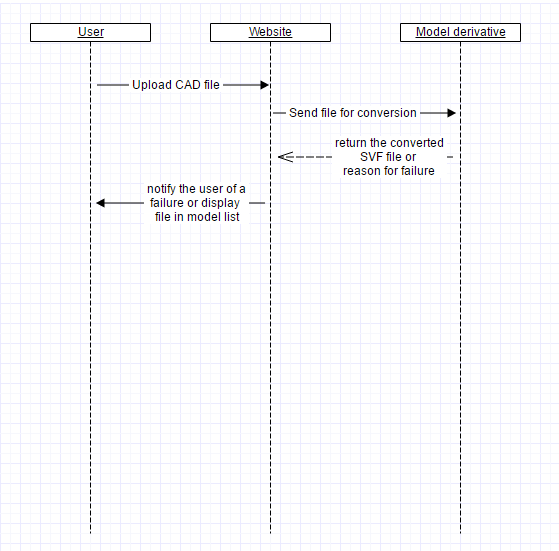
\includegraphics[scale=0.7]{conversionUML.png}
	\caption{File conversion interaction UML}
\end{figure}

\newpage
\subsection{Data Authentication}
\label{Two legged} 
	If there are resources a user can access without needing to provide permissions the 2 legged authentication system will address this. This takes use of the Forge's Data Authentication API and their OAuth rest points. The application will have a 32 character string that serves as the "client ID" and there will also be a client secret (which act as the password) both will given as a query parameter. 
\subsection{Interaction viewpoint for two legged authentication}
	Application requires resources from the Autodesk API and/or servers that do not need a users permissions. Application uses the POST authenticate endpoint to send client ID and secret along with any necessary scopes. Upon successful validation of credentials, access token is returned. When the token expires the process must be repeated.
\subsection{Design Concerns}
	The data must be secure and the exchange must be quick. A drawback of using Autodesk API and/or servers is the heavy reliance on it. The performance of the application is dependent on Autodesk, if the servers are slow or down, so is the application.
\subsection{Elements}
\begin{description}
	\item[]\textbf{Application} has a Client ID and Client Secret associated with it.
	\item[]\textbf{Client ID} acts as application username, 32 character string and passed as the client id query
	\item[]\textbf{Client secret} is the application password, 16 character string and passed as the client secret query
	\item[]\textbf{Access token} is returned at the end of a successful authentication flow, 28 character string used for subsequent API calls to the Forge platform. 
\end{description}

\begin{figure}[ht]
	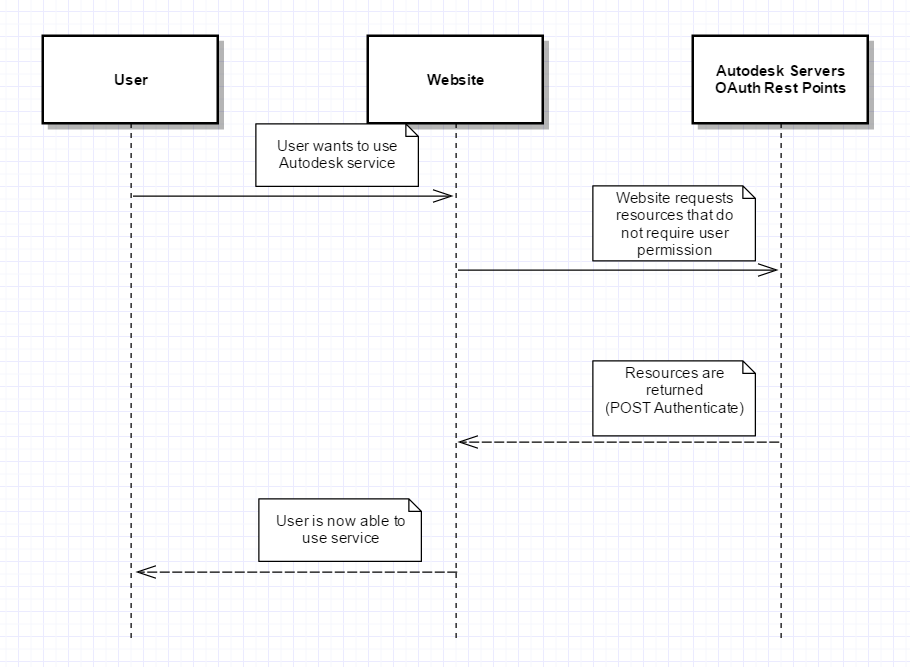
\includegraphics[scale=0.7]{Authentication2legged.png}
	\caption{Two legged OAuth UML sequence diagram}
\end{figure}

\subsection{Data Authentication}
\label{Three legged} 
	If there are resources the application requires that also require the permissions of the user. Then the 3 legged authentication will be used. This takes use of the Forge's Data Authentication API and their OAuth rest points. 
\subsection{Interaction viewpoint for two legged authentication}
	Application requires resources from the Autodesk API and/or servers that need a users permissions. Forge platform requires use of the "Authorization Code" grant type. User will be redirected to the Autodesk login (GET authorize endpoint). The user will have to register a new account if they do not have one. Then the user must explicitly accept the permissions the application requests. Using the callback URL the user is redirected to the application with a authorization code. With the code, client id and client secret, the application calls the POST gettoken endpoint. When successful the access token and refresh token are returned. The application is now able to obtain the resources needed. If the token expires the refresh token can use the POST refreshtoken endpoint to get a new access token. 
\subsection{Design Concerns}
	The data must be secure and the exchange must be quick. A drawback of using Autodesk API and/or servers is the heavy reliance on it. The performance of the application is dependent on Autodesk, if the servers are slow or down, so is the application. Three legged authentication also requires the login and permission of a user. If the user does not want or cannot provide permission then they are unable to use the application. Another concern is that the user must already own an account, if they do not they will have to create one. 
\subsection{Elements}
\begin{description}
	\item[]\textbf{Application} has a Client ID and Client Secret associated with it.
	\item[]\textbf{Client ID} acts as application username, 32 character string and passed as the client id query
	\item[]\textbf{Client secret} is the application password, 16 character string and passed as the client secret query
	\item[]\textbf{Access token} is returned at the end of a successful authentication flow, 28 character string used for subsequent API calls to the Forge platform. 
	\item[]\textbf{Callback URL} is the URL the user started from before they were redirected to the Autodesk login. It is necessary in order to bring the user back to the website.
	\item[]\textbf{Authorization code} is passed through the code query parameter when the user is returned to the application via the callback URL. Using POST gettoken endpoints as well as the client ID, client secret and this code, the application is able to receive an access token. The authorization code is 40 character string.
	\item[]\textbf{Refresh token} can use the POST refreshtoken endpoint to get new three-legged access tokens with having to have the user repeat logging in. Refresh tokens are 42 characters strings.

\end{description}

\begin{figure}[ht]
	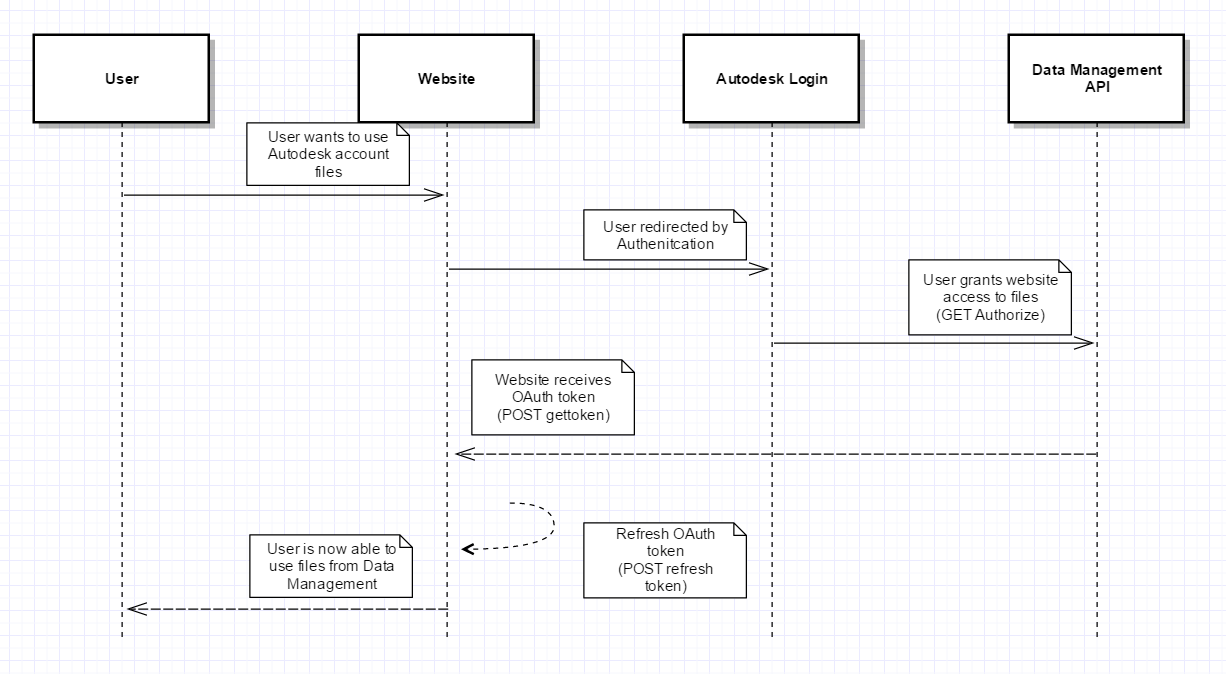
\includegraphics[scale=0.55]{Authentication3legged.png}
	\caption{Three legged OAuth UML sequence diagram}
\end{figure}

\subsection{Data Management API}
\label{A360} 
	A360 Personal requires 3-legged authorization for the application to access data. Then allows users to choose personal files for the application to use.
\subsection{Context viewpoint for Data Management API}
	In the flow the user wishes to access files from their A360 account. So to first do this they must login via the data authentication API. Once this is done the application is capable of using the resources from their A360 account. Next the users uses the data management API in order to choose the file they wish to use. 
\subsection{Design Concerns}
	Since all data that comes from A360 belongs to an account, it is assumed that a user first off, is registered and has an account. Furthermore, that the user logins in and through the Data Authentication API provides the permissions to the application to allow the use of A360's resources. Second is that files actually exist in the accounts storage, if there are no files the user has nothing to choose to use. If the user does not choose a CAD file this issue is not caught at this stage in the application, it is done later.
\subsection{Elements}
\subsubsection{Entities}
\begin{description}
	\item[]\textbf{Users} 
	\item[]\textbf{Data Management API} allows users to access files in their A360 for any sort of use.
	\item[]\textbf{Data Authentication API} provides the security and access of resources to the application.
\end{description}
\subsubsection{Relationships}
\begin{description}
	\item[]\textbf{User and Data Authentication's Relationship}: The user must login their Autodesk account and then provide explicit permissions for resources. This will give the authentication the okay to begin sending tokens. \ref{Two legged} and \ref{Three legged}
	\item[]\textbf{User and Data Management's Relationship}: The user will select the files they want from the data management and the data management API will provide those files to the user. \ref{A360}
	\item[]\textbf{Data Authentication and Data Management's Relationship}: The data authentication API will keep the token that allows the data management API to send resources to the application.
\end{description}
\subsubsection{Constraints}
\begin{description}
	\item[]\textbf{Users} must have a Autodesk account registered as well as files within the data management API.

\end{description}

\begin{figure}[ht]
	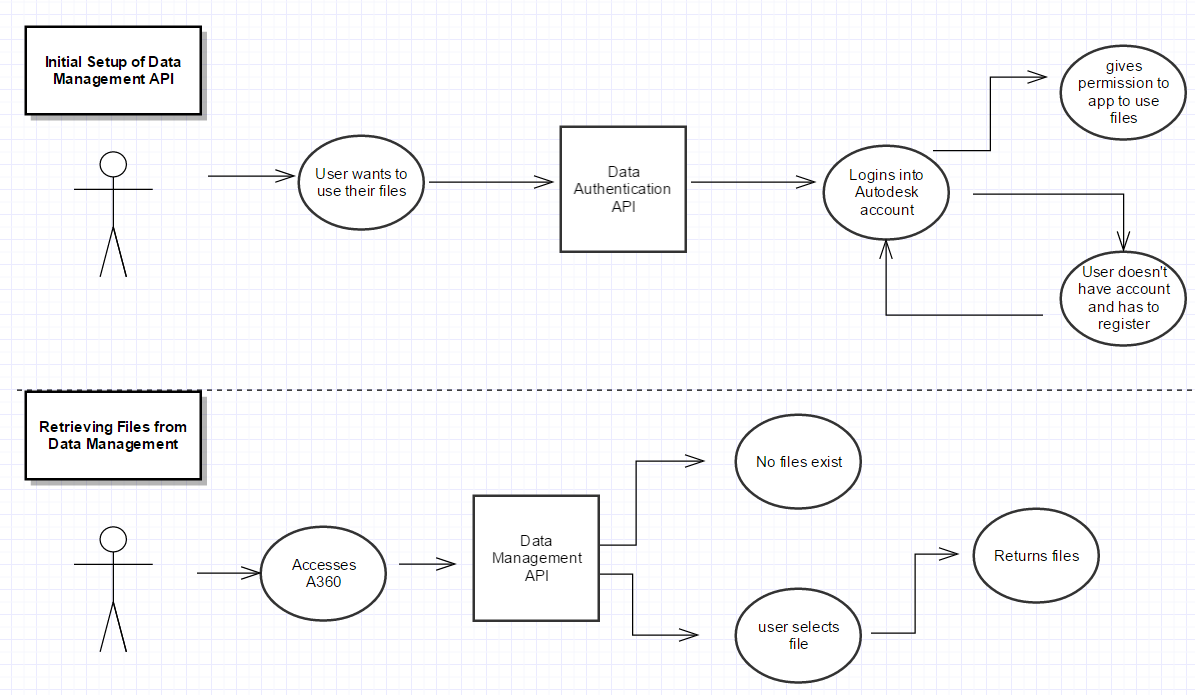
\includegraphics[scale=0.6]{DataManageUseCase.png}
	\caption{Data Management UML use case diagram}
\end{figure}
\newpage
\subsection{View models in VR}
\label{Mobile web based VR - Google Cardboard}
	The Google Cardboard application allows for web pages to be loaded into Android WebView. This uses WebGL for websites to be able to be viewed in the Google Cardboard's VR.
\subsection{Context viewpoint for WebView}
	In the flow the user wishes to view the model on the website on their mobile device and then use Google Cardboard in order to view the model in VR. In order to do this they utilize the QR scanner to get the website. Then to view in VR they open their Google Cardboard application. From there they use the WebView to view the site in VR which accomplishes their goal.
\subsection{Design Concerns}
	This design instance assumes that the user owns Google Cardboard and its accompanied application. Since the viewing experience currently uses Android WebView, the only mobile devices supported are Android devices. As WebView utilizes WebGL support, Android versions below Lollipop are not supported.
\subsection{Elements}
\subsubsection{Entities}
\begin{description}
	\item[]\textbf{Users}
	\item[]\textbf{The Website} displays 3D models.
	\item[]\textbf{The user's mobile device} The hardware on which everything happens.
	\item[]\textbf{Google Cardboard Application} has the WebView function that allows for the view of websites.
\end{description}
\subsubsection{Relationships}
\begin{description}
	\item[]\textbf{User and Website Relationship}: The user will scan the Websites QR code. The website will now display in the users device.
	\item[]\textbf{User and Google Cardboard Application Relationship}: The user will open the application and the application will begin to run.
	\item[]\textbf{Website and Google Cardboard Application Relationship}: The Google Cardboard application will take the website and put it through the WebView function, resulting in the Website becoming viewable in VR.
the application.
\end{description}
\subsubsection{Constraints}
\begin{description}
	\item[]\textbf{The user's mobile device} must be Android and Android version Lollipop or higher. 
\end{description}
\begin{figure}[ht]
	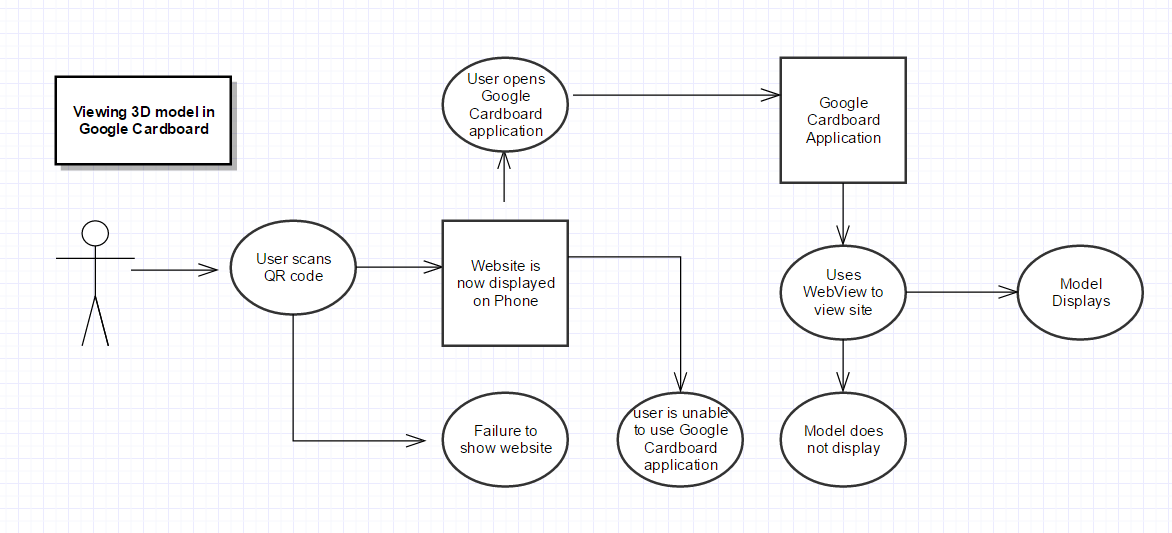
\includegraphics[scale=0.6]{ViewingUseCase.png}
	\caption{Model Viewing on a mobile device UML use case diagram}
\end{figure}

\newpage
\section{Design Document Changes}
Instead of creating our own login, we decided to adapt the NPM library created by Adam to aid in the process of using the Forge API. This was also done for the non-local file upload. In fact, most areas where the API were being used this NPM library was utilized. This was due to several factors, first the person who created the NPM library was actually an Autodesk employee that Kean could put us in contact with. Second, instead of writing our own version, we could use this library to save time. Finally, using his code would be much more stable. 

\newpage
\section{Technology Review}
\thispagestyle{FirstPage}

\bigskip

{\centering\selectlanguage{english}\bfseries\color{black}
Technology Review
\par}


\bigskip

{\centering\selectlanguage{english}\bfseries\color{black}
November 10 2016
\par}
\bigskip
\bigskip
\bigskip
\bigskip
\bigskip
\bigskip
\bigskip
\bigskip
\bigskip
\bigskip
\bigskip
\bigskip
%\begin{center}
%	
\includegraphics[scale=0.8]{forge_logo.png}
%\end{center}


\vfill
{\centering\selectlanguage{english}\bfseries\color{black}
Abstract
\par}

{\centering\selectlanguage{english}\mdseries\color{black}
	The Forge VR Explorer branches from an Autodesk prototype project called Vrok-It, which is a simple web-based 3D 
	model viewer and mobile virtual reality (VR) explorer. The project will expand upon its ability to display uploaded 3D 
	models in browser and in VR, and improve its accessibility. Conventionally, viewing 3D models in VR is a challenge if 
	you have model files on many devices, or have a headset that only works in conjunction with a smart-phone. The 
	Forge VR Explorer aims to do this by utilizing a web-based software that uses the features of the Autodesk Forge API. 
	The project will also be expanded with new ideas and stretch goals as the project is developed.
\par}
\clearpage

\section{Introduction}
	The Forge VR team (group 20) will be working building on the Vrok-It project. We will be trying to make the site more accessible for users
	as well as trying to increase the performance of the  of the viewer and the VR experience too. Shawn Cross will be tasked with the file
	uploading feature, file conversion, and connecting the users device. Griffin Gonsalves will be working on the Website UI Redesign, Data Management API
	and Model Viewer. Paul Kwak is going to be working on Forge Authentication, Viewing in VR, and hardware detection.
	
\section{Technologies}

	\subsection{File Uploading}
		\begin{enumerate}
			\item{Options}
				\begin{itemize}
					\item  Use a plug-in: Using a plug-in that would handle file uploading would be very convenient as it takes a lot
						of the work out of it. One of the  biggest benefits would be that this could save us a lot of time. If we were to use
						the plug-in we would not have to worry about the effort that would normally go into creating our own, we could simply just
						find one that would fit  what we needed and the put it into our website. However this does also lead to the problem that we
						may not be able to find one that exactly fits what we want. Many of the plug-ins I have found so far simply upload the file to
						a server and then it is done. In our case we need the file to be usable by the website once it is uploaded.
 
					\item  Create our own file upload feature: Creating our own uploading feature would allow us to make the feature 
						work exactly the way that we would want to. Their a many different ways to do this though. One common way I have found 
						is to first create a web form using HTML to make the upload button.Then you could use PHP to submit the file through a POST.
						Using AJAX and JQuery you could also add features that show the progress of the upload and verification such as verifying correct 
						file types are being used. This could take a lot more time and effort to complete though depending on how skilled the person creating 
						the upload feature is and how fancy they want the feature to be.      

					\item  Create our own file uploading feature using new File API added to HTML5: This is similar to the previous option but seems like it might 
						be easier to learn and understand. Many of the features that we wanted are built into the API making it easier for us to create the 
						upload file file feature the way we want it. Though there will be some time for learning how to use the API and some time to completely
						create the feature, there is a lot of good documentation on this API that should make the process go smoothly.  
				\end{itemize}
			\item{Criteria being evaluated}
				\begin{enumerate}
					\item How much time will it take to integrate into our project: The plug-in will definitely take the least amount of time to add this to the project. I 
					think that the other two options will both take more time to do since you will have to create the upload feature from scratch.
					\item How much effort will have to go into learning how to complete the task: The plug-in won't take a lot of time to learn how to use since you just 
					need to add the library to the project and then you can use it. The other two options will take more time to learn how to do but shouldn't be to much 
					time since there is a lot of documentation and examples on-line showing how to do this. 
					\item Will the upload feature do exactly what you wanted it to do: If you aren't really particular about what the file upload button looks like or how it shows
					the progress of the upload then the plug-in would work just fine. However if you want to make the upload button look a certain way and show its progress a
					certain way then one of the other two options is going to be best. 
					\item Which option will offer the most secure way to upload the file: All three options offer the same amount of security. 
				\end{enumerate}
			\item{Discussion:} The plug-in option will definitely save the most time in terms of learning it and getting it to work in on the website, 
					however it will likely give you little in the way of customizing and making the file upload feature work exactly how you would want 
					it to. Both of the options to make you own file upload feature will result in a longer time to learn how to do this as well as a longer
					time to complete the task. This does allow you to make sure the the file upload will do exactly what you are wanting it to do. the 
					third option will is also using HTML5 this means that is will work in all the new browsers.
			\item{Select Option:}
					 I believe that the extra time that it takes to create our own custom file upload feature will outweigh the extra amount of time 
					that it will take to do this. I also think that the use of the file API is better since it is well documented, easy to find examples
					for, and has many of the features that we wanted built into it.
		\end{enumerate}
	\subsection{File conversion}
		\begin{enumerate}
			\item{Options}
				\begin{itemize}

					\item accusoft API:~\cite{accusoft2016} This is an API that allows users to convert their CAD files in to raster files such as SVG (scalable vector graphic) files that could 
						to view in the model viewer. This API does cost money and depending on how many conversions the user is planning on doing this option
						could turn out to be relatively expensive. There is a lot of documentation on how this API can be integrated into an application but it seems
						as though the integration process could be harder if you are not using a certain types of applications.

					\item  Forge Model derivative API:~\cite{forge2016} This API has the ability to take users CAD source file and convert them into OBJ and STL files. This API can also
						convert the files directly into SVF files the same type of file that the model viewer API we will be using on this project uses. This API would 
						also not cost us anything to use while we are working on the project since the company that created the API is the same company we will 
						be making the project for. There might be a little bit of a learning curve when it comes to integrating it into the website but the API has a 
						lot of tutorials and documentation on how to use the API in an application.  This API also uses a token based authentication system that
						provides security when converting the users files. 

					\item  cloudconvert API:~\cite{cloudconvert2016} This API gives you the ability to convert from CAD source files to a SVG file but it also give you the ability to convert the 
						other way was well. This API also has well documented instruction on how to integrate this API into an application. That would make it easier
						to learn and take less time to complete the task. This API would cost money to use depending on how much time is spent doing the conversions.
						this one also requires that a key be used when doing the to be created which make this more secure to do file conversions on since it will be able 
						to verify that it is an actual users trying to do conversions. 

				\end{itemize}
			\item{Criteria being evaluated}
				\begin{enumerate}
					\item How much time will it take to integrate into the project: All three of the projects will take about the same amount of time to integrate into the 
					project. I think that the first option might take longer since the documentation looked like it might be hard to understand and didn't seem as accessible 
					as the other two APIs. 
					\item How much effort will have to go into learning how to complete the task: I think each of these could take a good amount of effort to understand how
					to use and set up. Options two and three seem to have easier to understand documentation and have more example of how to use the API. 
					\item How secure is the file conversion: The first API didn't say whether or not that it had a way of making sure that the file conversions were secure.
					Options two and three both had some sort of way of authenticating the conversion. Option two used a token system and option three used a key system.
				\end{enumerate}

			\item{Discussion:} These three options all offer similar conversions. They all convert the CAD source files into a usable file for the model viewer. The Forge API will however 
				convert the file into an SVF file that can then be directly loaded into the viewer. This could save time and make it easier to complete the task. The Forge API is also 
				free for us to use during the duration of the project so that would also make a big difference as well. Finally the Forge API offers the most secure option when it comes
				to converting the users files since it  requires a token authentication to even do the conversion. This token is created as soon as the user visits the website and last for 
				the duration that the user is on the website. Also with lots of documentation as well as tutorials on how to integrate the API into our application I feel like this option will
				take the least amount of time to complete the task. 

			\item{Select Option:}
				I Think that we should use the Forge model derivative API since it seems the most straight forward on how to integrate it into our application. It won't cost us any money
				to use and has a more secure way of converting the users files. 
		\end{enumerate}
	\subsection{Connecting the users device}
		\begin{enumerate}
			\item{Options:}
				\begin{itemize}
					\item Use a QR code plug-in: jquery.qrcode.js is a jquery plug-in that generates a QR code which can be scanned by a user to using a QR scanning application on
					their device to connect their device to the current web session. Using this would be relatively easy since we would just need to add the library to our project. That
					means that there wouldn't be a lot of learning time involved in using this option.

					\item QRickit API: This API can dynamically generate QR codes to be used in a web/mobile application. The API is free to use for personal and small business 
					applications so there would be no cost for us to use it with our project. There is also documentation on how to setup and use the API so this would cut down 
					on the time that it take to learn how to integrate it into our project. 

					\item QR Code Generator: This is another API that will that will generate a QR code for the us. It can easily be embedded into the web page by putting the 
					source into an image tag. This API also allow for you to specify how big you want it and allows for different backgrounds to be used. The API also Has all
					the documentation that is needed to set up and use so the time to integrate this API into the project would be much.  
			\end{itemize}
			\item{Criteria being evaluated}
				\begin{enumerate}
					\item How much time will it take to integrate into the project: I think that all of the options can pretty easily be integrated into the project. all have 
					documentation that clearly describes how set-up and use them. Overall I would say that each of them are about the same when it comes to the 
					amount of time that it will take to integrate them into our project.  
					\item Will there be a lot of learning involved in using the option: I also feel like that since each of these options has documentation describing how to 
					use each that the learning involved in each is pretty minimal. 
					\item Will it connect the users device quickly: each of the should have about the same time to connect the device. The only reason that there would be a 
					slow down in connecting the users device is if they had a slow Internet connection or if there was a lot of traffic on the website itself. 
				\end{enumerate}
			\item{Discussion:} Overall I think that all the options are pretty close to one another. All three of the options are pretty straight forward in terms of integrating them
			into the project.  All three should also connect the users device quickly. The two API options add the ability to customize the QR code, but that really isn't needed for 
			our project since we just need the QR code to be there so the user can connect their device. 
			\item{Select Option:} I would say that the plug-in is the best way to go since we can integrate the library directly into our project and not have to worry about making 
			any calls to an outside API. 
		\end{enumerate}
	\subsection{Website UI Redesign}
		\begin{enumerate}
			\item{Options}
				\begin{itemize}
					\item{WordPress}
					WordPress is a high-level framework that can generate a simple view for a website. Wordpress has the advantage of using many pre-created templates in order to display a page. Wordpress is highly supported by many browsers, and could simplify the process of creating updates to the site. There is also the added benefit of a very pristine looking webpage without spending too much time developing it.
					\item{AngularJS}
					Redesigning the entire site does not require starting from the ground up. We can implement a javascript framework that would help us organize and manage the site. Angular JS would assist us in creating a better interface for the website without that much learning required. Our project is already using javascript to handle much of the project operations, but implementing a framework for the interface should not conflict with the rest of the project. Angular is completely free and has plenty of documentation available. There is also the newer edition named Angular 2, but due to the complexity, it may not be advisable to use.
					\item{ReactJS}
					React JS is another javascript framework that can generate different views for the page from a special source file. It simplifies javascript programming, in addition to generating simplified code for the project. React is also completely free, and has plenty of documentation and tutorials available online. Mobile browsers also are supported by React.
				\end{itemize}
			\item{Goals}
			Improve site layout and visual appeal
			\item{Criteria being evaluated}
				\begin{itemize}
					\item{Development time:  Each different option would potentially take different amounts of time to complete-potentially much longer than we have time for. Evaluating how long it will take to implement is a necessity.}
					\item{Presentation: This would be the look and style of the option. Specifically, whether it looks nice or not.}
					\item{Learning curve: Having to learn a new framework for web development could take weeks of time. This also factors into the development time.}
				\end{itemize}
			\item{Discussion}
			Each option provides the advantage of creating a nice interface, but each does so at a cost. Angular could take the longest to learn, and could also be difficult to implement. React has the advantage of creating nicer interfaces at little overhead. It certainly is the most different and could be a challenge to learn, but the resulting pages could bet a great choice for the project. Wordpress, though convenient, will not be able to keep up with our project, and would be challenging to continually update the layout with each change to the project during the development phase.
			
			\item{Select Option}
			In weighing the options, using ReactJS would be the best option for the project. Because the site already has a working page, we think it would benefit the project more to spend less time developing the updated UI and more time on the focus of our project. After learning the basics, ReactJS should provide a great interface for our website that improves our development process.
		\end{enumerate}
	\subsection{Data Management API}
		\begin{enumerate}
			\item{Option}
				\begin{itemize}
					\item{Forge Data Management API: Belonging to the Forge collection of APIs created by Autodesk, this software allows for the user to pull project files from an Autodesk A360 library that contains a user's project files. These files could be filtered and shown in a user interface, which is a criteria for this technology. Once a website is registered with the API, and a user is logged in, files may be accessed in the interface.  The usage of the API is straightforward, after setup with the API, we would only need to include a provided configuration and setup on the site which could assist in rapidly developing this feature.}
					
					\item{OneDrive API: Another common cloud service is Microsoft's OneDrive. Microsoft provides a File Picker API through their Javascript SDK, which is also the main scripting language used in our project. After registering the app with Microsoft's API, one may implement a "Open from OneDrive" button which opens a File Picking window where the user may pick a file from their drive. This API would support all major web browsers, in addition to the most current mobile browsers. This API should have no problem integrating with our other assets, and provides a UI popup for selecting the file.}

					\item{Google Drive API: A similar, but more general use case API that fits the bill is the Google Drive API. This API lets a user log into their google account and access their files stored on Google Drive. Google claims the API works flawlessly in a straightforward HTML web document, so compatibility should not be an issue with other components in the project. Furthermore, since the API supports the viewing and interaction with user's files in an interface, the API meets the criteria of having an interface. This interface, called the Google Picker, functions as the interface for picking the file.}
					
					
				\end{itemize}
			\item{Goals}
			To provide an alternate method of file upload to the project through a cloud service.
			
			\item{Criteria being evaluated}
			\begin{itemize}
					\item{Level of browser/device support: How many modern browsers does the technology support?}
					\item{Project asset/Website compatibility: Does the new API work with the rest of the website?}
					\item{File picking user interface: Does the API's user-interface function for our project?}
				\end{itemize}
			\item{Discussion:}
			This sounds like a cut and dry choice for the Forge API, as we are already using Autodesk APIs and libraries on the site in addition to other Forge components. Using this API could save development time as the app need only be registered with the Forge service once, and appears relatively trivial to implement in the site. The Microsoft API seems useful, but the OneDrive cloud service is not oriented to provide large files on demand, and configuration seems much more complex. On the other hand, the Google Drive API seems like it could be a suitable backup. The functionality seems slightly more complex, however this would provide cloud access for users on the most used cloud platform.
			\item{Select Option:}
			Due to the inertia behind our project using the Forge Collection, I think the best option for the project is to include the Forge Data Management API. It meets each of the criteria for the project and should function as a useful feature when completed. 
		\end{enumerate}
		
	\subsection{Model Viewer}
		\begin{enumerate}
			\item{Option}
				\begin{itemize}
					\item{Forge Large Model Viewer: This is the current system in place for the project. Created by Autodesk, the LMV allows for larger project files to be viewed and manipulated in-browser, and on mobile for most modern smartphones. The viewer is placed in the web document as a window.}
					\item{WebVR Rendering: A very new initiative from Mozilla that provides high performance graphics on the web aimed at supporting many new VR devices, including Google Cardboard. The system supports different mobile devices and is also supported on mobile web browsers. The software is implemented within the project as a library. }
					\item{Unity 3D: Unity provides another method of 3D model viewing for browsers. The Unity Web Player is capable of detailed 3D projects in a web browser, including full 3D games, models, and more. Unity has also recently provided support for the Oculus Rift. However, the software is built upon the same OpenGL renderer as both WebVR and the LMV. }
		
				\end{itemize}
			\item{Goals}
			Provide a viewing interface in which to view a 3D model in-browser.
			
			\item{Criteria being evaluated:}
			
			\begin{itemize}
					\item{Model Quality:}
					\item{Web Viewing Experience}
					\item{VR Viewing Experience}
					\item{Device and VR system support}
			\end{itemize}
			
			\item{Discussion:}
			There is a large project codebase that was built on top of the Large Model Viewer specifically for the project. Moving to a different 3D/VR framework would take considerable work and commitment for the project as a whole, but could potentially bring more support and features to the project that we could use. WebVR by far seems the most advanced, high-quality and broad ranging in terms of device and browser support, but with the disadvantage of having nearly no documentation or tutorials. Unity provides a very easy to use web model viewer, but only has support for a single VR headset, which would fail to meet the Device and VR system support criteria. 
			\item{Select Option:}
			Currently the best option for our project at the moment would be the Large Model Viewer. Granted that both webVR and Unity support high quality models that can be inpsected closely, the amount of the project that currently relies on the LMV would be too large of a task to make the jump to a newer framework at this point given the alternatives. Through communication with our sponsor, we may be able to use a different framework later down the line, as there could be a new API to use. Currently, it does not seem sufficiently justified 
	\end{enumerate}
		
	\subsection{Forge Authentication}
		\begin{enumerate}
			\item{Option}
				\begin{itemize}
					\item OAuth2 is the open standard used in the Forge platform for token-based authentication and authorization. The basic flow for using OAuth commonly begins with an application making an HTTP call to a OAuth REST endpoint and providing its credentials. A token is returned to the application and then subsequent HTTP calls to various APIs on the platform include the token in the request header.
					\begin{itemize}
						\item Two-legged authentication: The default and simplest type of authentication. Should be used when an application makes a call to an API that utilizes resources that do not require the user's permission. The only interaction is between the application and the Forge platform. The user does not need to know about the authentication or provide authorization to the application for resource access.
						\item Three-legged authentication: Used for when an application requires access to resources belonging to an end user, and so that user must provide explicit authorization. For a web application, this will automatically redirect to an Autodesk login page and ask for the user's consent. Then the user is redirected to the application, which is now capable to accessing those resources
					\end{itemize}
				\end{itemize}
			\item{Goals} provides security to data interactions and also to resources that belong to users being exchanged.
			\item{Criteria being evaluated}
				\begin{itemize}
					\item{Whether users will need access to Forge resources}
					\item{Usability, users have to login and have an Autodesk account}
				\end{itemize}
			\item{Discussion} There is a slight possibility to be using both. Two-legged for simple users and then three-legged for users with Autodesk accounts. Regardless of whether we accommodate simple users, we definitely will have to use three-legged. This is due to the use of the Forge Data Management API, users who store their files will be using the Forge platform. Thus will have to have users verify our application the permissions to access their files. As for the use of two-legged that will vary depending on what other pieces are added.
			\item{Select Option} : The functionality of the Forge Data Management API revolves around users files so we will definitely have to utilize three-legged.
		\end{enumerate}

	\subsection{Viewing in VR}
		\begin{enumerate}
			\item{Option}
				\begin{itemize}
					\item
					Google Cardboard: Costs \$15. Turns any mobile device into a 3 dimensional viewing environment. Putting the phone into the contraption and using compatible apps allows a VR viewing experience. When porting in model files via QR code the issue is getting the files into format that makes them VR. There are a number of applications available for free that do this so the process might be very simple and definitely already exists.
					\item
					Costs \$599. A mobile VR viewer already exists that has CAD file viewing. However, costs money to use and is still a work in progress. Porting Solidworks CAD files directly into Unity is possible and works but does not utilize the flow we are using. Another avenue with might be to use an application under the sketchfab VR umbrella.
					\item	
					Costs \$1,500. Requires a PC to either view on, but also requires the user's phone to have bluetooth if the user wishes to use the phone. With this option also changes the flow for the project. CAD files can be exported from Solidworks into a .3DS format. The .3DS format can be directly imported into Unity which then has Vive support and allows for viewing via that. 
				\end{itemize}
			\item{Goals} display our adjusted model in VR while maintaining the smoothest possible viewing experience.
			\item{Criteria being evaluated}
				\begin{itemize}
					\item
					Cost/Accessibility
					\item	
					Documentation for each
					\item	
					How well does it fit within our established system.					
				\end{itemize}
			\item{Discussion}: Google Cardboard has several advantages. First off it's incredibly cheap price, will allow for greater accessibility. Especially for developers, each us will be able to use our own and testing models should be easy. Second is the high number of application that display models and their easy access (free). This gives us an easy way to compare our work, framerate wise. Finally since our current setup utilizes Vrot.it and already had a QR scanner to port the models to our phones. It becomes a matter of adjusting the model and then using the VR format Cardboard uses to get our desired VR model. Oculus and Vive come with the advantage of having higher hardware to work with. Our need to detect hardware becomes less of an issue since both work with PC's and then display to the phone via other methods. This comes at their high cost and additionally the applications out for those options don't utilize our current setup. In fact would change our setup completely since they alleviate the need to even upload files and just change our problem to converting CAD files to work with Unity. 
			\item{Select Option}: Google Cardboard is significantly cheaper and perfectly fits within the way we have setup in order to utilize what we have. 
		\end{enumerate}
	\subsection{Technology 9}
		\begin{enumerate}
			\item{Option}
			\item{Goals}
			\item{Criteria being evaluated}
			\item{Discussion}
			\item{Select Option}
		\end{enumerate}


\section{Conclusion}
After our technology review, we have made some important evaluations on our project and its different components. For many components, we decided it was best if we continued using some of the technologies from the original project, in addition to focusing on utilizing new API's and frameworks that fit the goals of our project. We are planning on potentially adding an updated version of the Forge Large Model Viewer that is currently being developed.

\newpage

\section{Technology Review Changes}
Yes we changed our mind about one technology in particular, we were essentially going to have to start from scratch and just write everything ourselves and/or adapt smaller projects. Instead we found an NPM library with all the API prebuilt for use. We decided to utilize this over the option of writing from scratch. For the advantages of saving time and having a more stable foundation to built upon.

\newpage

\section{Weekly blogs}
\subsection{Fall}
\subsubsection*{Week 3}\hspace*{\fill} \\

Shawn Cross

This week we were able to get in contact with our client Patti and have a couple of conference calls with her. After the first call we began to come up with problems that we might be able to solve using the Forge Api's. During the second call we met with Patti and Jim Qaunci and went over the list of ideas we had come up with during the week. During that call we were able to begin narrowing down what it is we were going to be doing for our project. One of the biggest problems that we have encountered so far was not really knowing what it was that we would be doing for this project. We were also having trouble trying to figure out problems that we could solve using the forge API technology. For next week we will be finishing up our problem statement to be signed and starting to on the next step of the project.\\

Griffin Gonsalves

This week, our group convened and tried to formulate some new ideas and talk about problems we could potentially solve with the Forge API. We spent a few hours each on a concise list that we were able to get feedback on from our sponsor, Patti Vrobel along with Jim Quanci who is working on the Forge API. We communicated through conference calls on Monday and Friday.

After getting acquainted we discussed some of our ideas and what would be best for the project as a whole. Jim brought in(via web) a couple of interesting projects from engineers at Autodesk to show us. From this we could see a demonstration of a creative application of the API, which was very useful to us as trying to narrow down and define our project has been the most significant challenge so far. One such solution would be to use a Virtual Reality, or Augmented Reality hardware solution to be able to make a 3D model viewer for one or more of these headsets. We liked the idea, and are planning on potentially making a draft of the plan. Moving into next week we hope to complete our project statement draft and abstract draft early in the week, and finalize our initial goals.\\

Paul Kwak

This week we had two meetings with our client, Patti. In the first meeting on Monday, we introduced ourselves and then began the talks on clarifying our project. The description of the project was 100\% what they wanted, literally anything utilizing the Forge API. After clarifying that we got some logistics issues solved, reports about how to convey our experiences using Forge. After the meeting we had a new goal of coming up with ideas about how we could use Forge API and make our project. We reconvened on Friday this time with Jim, who helped us narrow down our ideas or informed us of their difficulty. In the end he showed us a previous hackathon project that allowed for the upload of 3D models. Then presented the idea of being able to increase or decrease the detail of the models to allow lower end virtual reality to use less graphical power. Or for higher end VR devices to display models in higher quality thus fully utilizing the full power of a higher end VR device. Next week we need to finish out our problem statement and begin understanding the hackathon project as well as the Forge API.

\subsubsection*{Week 4}\hspace*{\fill} \\
Griffin Gonsalves

This week went smoothly and quickly. We were glad to be able to have a conference call with Patti, our sponsor, and worked out some more details for what would be the focus of our project. We each wanted to be able to have flexibility and the ability to add more ideas to the project as we developed. We were also able to update and get some feedback on our draft, which should help us create a great document for our project. During week 5, we are planning on completing the final draft of our problem statement. We are aware we are still a little behind, so we want to shift focus on our requirements document after we finalize our statement and request signatures. We were also able to get in contact with one of the engineers behind the vrok.it project, Kean, who is available to help our team on the project. We are planning on communicating more as we progress through our stages of planning. Overall, I'm excited for where we are headed as a team, and where our project will take us.\\

Paul Kwak

This week we only got 1 meeting with our client, it wasn't a incredibly productive meeting and was rather short. However, we did get contact information with the person who wrote the code for Vrok.it which should help us immensely. Unfortunately we won't be able to meet with him via conference call and only have email as a source of communication. This will really set back our progress on writing the problem statement and even on writing requirements since Kean, our contact, will be helping us narrow this and is unavailable. Next week we'll be trying to use email the best we can to find out what we need in order to complete our documents. If we aren't able to get enough details we may have to ask for an extension. All of agree that hopefully we'll be able to since getting behind on the documents will hurt us greatly.\\

Shawn Cross

Next week we plan on having the final draft of the problem statement done and signed by our client. We also plan to begin writing up the requirements documents as well. I look forward to deciding exactly what we will be doing and figuring out how we plan to it. I don't feel like we made a ton of progress this week however, we were able to come to an understanding of what it is we will be doing for our project, we just need to decide on the exact details. I think the biggest problem we encountered is the same one that we had from the week before. We just weren't sure exactly what it was that we were going to do for our project and that was making it hard for us to really write up a good problem statement. Now that we have a better idea of what it is we will be doing I believe that the documentation process go smoother.\\

\subsubsection*{Week 5}\hspace*{\fill} \\
Griffin Gonsalves

We made some good headway this week with our documents after finishing and signing our final statement on Wednesday as well as creating our first draft of our requirements document. I spent a lot of time working on the documents this week, and I think the problem statement turned out well. As a group, we've started to get a better hold on the project, and are tackling tasks a bit faster. Next week, we hope to get some feedback as well as meet with our client and associated people to create some specific functional and non-functional requirements. I'm glad we have caught up on a lot of work, and I think after we meet with our client again, we will be able to progress with clearer goals.\\

Paul Kwak

This week we finished up our problem statement and got our client to sign off on it. While we did not have a meeting with our client we instead met up as a group and began some more serious talks on breaking down our requirements document. We got a general outline of what we need to write and have a couple requirements. However, at a in person meeting on Friday we are going to create an email to address questions we have to Patti, Jim and Kean. Next week, we should have a client conference meeting and then also begin fleshing out the requirements document much better once we have more details and a better understanding from our client.\\

Shawn Cross

Next week we plan on having another conference call with our client to discuss the requirements document that we are currently drafting. We plan on taking their feedback and comments and use them to revise our first draft of the document. This last week we were able to finally get our problem statement finished and I feel like we are finally getting caught back up. We were also able to get together and start working on the rough draft of the requirements document. We didn't have as many set backs this week. With the information we received from Kean we were able to start to better understand what it is we are trying to really accomplish on this project. We did still run into a couple problems trying to figure out if some of the things we want to do on the project were actually feasible for us to accomplish in the time that we have so we decided to leave those out for now until we could talk to the client about them during our next conference call.\\

\subsubsection*{Week 6}\hspace*{\fill} \\
Shawn Cross

In the coming week we are hoping to get a chance to have a conference call with our client get the last of the questions we have about the project answered. We are also planning to have the requirements document finished, reviewed, and signed by our client. I aslo believe that we will be starting our tech reviews so I hope to get started on that as well. We were able to get most of our requirements document finished this week with a few more things to do once we are able to talk to our client. I also feel like this week we really started working together as a team a lot better. The biggest dificulty that we ran into this week was not being able to meet with our client and have our the last few questions we had about the functional requirements answered. however even without talking to our client we were able to get a lot of the document filled out.\\

Paul Kwak

This week were not able to meet with our client. However, instead we plan to meet with them hopefully with our TA Nels if possible to help clarify some details. I believe there were a couple issues with pushing to the github that happened we resolved those quickly. We met together on last Friday work on the Requirements document and this week filled in more details. However, it seems we will need more time to finish out the Requirements document. There are tons of sections that aren't quite clear and may or may not apply to our project. Furthermore, more details have to be expanded upon by our clients. While we have a Gantt Chart Template we will probably try to fill that out next week along with finishing the requirements document.\\

Griffin Gonsalves

This week I spent a good amount of time editing the requirements document in Latex, fixing and adjusting our format and content based on feedback from Tuesday's lecture. We made more changes Thursday and Friday, and we are picking up some steam! Hopefully once we we complete more of the document we will also be able to complete our Gantt Chart we began. We wanted to meet with our client this week, but are still awaiting a response. Overall, we have a better idea of some of the tangible requirements we would like to pursue which has helped bring a bit more cohesiveness to our project. By next week I hope that we have reached out to our client for additional guidance on the project and our requirements.\\

\subsubsection*{Week 7}\hspace*{\fill} \\ 
Griffin Gonsalves

With having our first version of our requirements doc out for feedback, we are finally able to look back and make adjustments that will help our development process. From feedback we found some components that we need to include in the final document. We would need to authenticate the app with autodesk's API in order to allow for autodesk users to log in to our web app, and use their cloud files. This is required for using the model derivative API and the data management API, so we made sure to update our document. We also included our Gantt Chart, which features our major goals, components and estimated time frames for our completion. We began our Technology Review earlier in the week as well, deciding our components we will be responsible for and some ideas we had for the document. I think our technology review is fairly straightforward, and will help us see any other technologies we haven't considered yet.\\

Shawn Cross

This week we were able to finish a draft of our requirements document and get feedback from Nels about the changes that we should make to it. One of the biggest suggestions he had was to be more detailed in the description of our functional requirements. We were also able to get ahold of our client Patti this week and should be having a conference call with everyone sometime next week. I believe that this call will be very helpful and we will be able to get a lot of our questions and concerns answered. This week we have also started our tech reviews which is an individual assignment which is meant to help us to find which technologies will best work for our project. Next week we should have these tech reviews done and turned in. I also hope that next week we will be able to get a jump start on the design document and clear up anything we are still unsure of for this project. I don't think we ran into to many problems this week. We were having some trouble with the formatting of our latex file but after talking to Nels we realized that we were just making it harder than it needed to be.\\

Paul Kwak

Being sick for most of this week I was unable to do as much as I was very sick. I was able to create a much nicer Gantt Chart from the draft we made last week. Due to my sickness I wasn't able to meet with Nels or my groupmates, we do have our assignments for the tech review so I will be working on that to have done for next week. Patti is trying to get a meeting setup with all the current members together so we can have a sit down call and work out questions and clarifications. I'll be working hard to make up for the work I wasn't able to do this week with the last of the documentation coming up in the last weeks of the term.\\

\subsubsection*{Week 8}\hspace*{\fill} \\
Griffin Gonsalves

Despite the hectic week, I was able to complete my portion of the Tech Review. I was tasked with reevaluating several sections of the existing base project, namely the Model Viewer and the Data Management API. I was able to compare the technologies we might be using against each other and make a decision on what would benefit the project more. It was quite time consuming, but rewarding as I was able to learn more about our projects internals as a result. The last technology I reviewed was our Website's Interface. I researched ReactJS, which is capable of implementing an easily modified and widely supported web framework and saw it had very strong potential for the project.

We are hoping to meet with our client on Thursday. During this meeting we have quite a bit to cover since we had some difficulty connecting in weeks prior due to schedule conflicts, and travel. Our goal is to verify that our technologies are feasible and benefit the project. Additionally, the team and I are planning on beginning our design document as soon as possible.\\

Shawn Cross

To begin this week we had to have our tech reviews finished. This assignment was mainly an individual assignment but also required that we merge all three of our parts into a single document that flows nicely. Even though the tech review did take me quite awhile to do I found it very useful. It helped me to better understand many of the components of the Vrok-It project that we will be starting with. It also helped me not only helped me decide on how I want to implement my tasks on the project it also helped me find things I think I could improve on the current project. We are also beginning to work on our design document for the project. I am hoping to get a good chunck of this done by the start of next week so that we will have time to get feedback on it and revise it at least once before it is due. To end this week we are getting a chance to have a conference call with our client Patti and the other people involved on the project. One problem I ran into this week was trying to get the bibtex to work in our latex file. After messing around with it for awhile I realized that I was just making some dumb mistakes and was finally able to get it all working. I was also having some trouble trying to find different APIs to use instead of just the forge API for converting files, but after doing some research I was able to find a couple that had similar functionality to the forge API. Next week I am hoping that we can get most design document done since I should have some extra free time with the long weekend.\\

Paul Kwak

I got two out of the three section I had to get done. This was mainly due to the lack of information regarding detecting hardware. There are tons applications for doing this and many manual ways to do this for a singular user. I really need help as it feels like Google only turns up the applications and the manual ways of doing this. Also while searching for ways to view in VR, there appear to be some applications that are specifically designed for doing what we are attempting to do. Including the website to device viewing on some applications as well as the CAD files capability. We'll have a big meeting with Patti, Jim and Kean on Friday hopefully and get to work on the design document early. I've been dragging slightly on my end but will be doing my absolute best to not affect the team in anyway.\\


\subsubsection*{Week 9}\hspace*{\fill} \\
Shawn Cross

With the holiday this week was not as productive as I had hoped it would have been but I also expected that because of the holiday. We were able to get the Design document started and I think we should be able to have a good portion of it done by the end of the weekend. Each of us are going to try to tackle different prat of the document. We also had another conference call with Patti this week and were joined by Kean and Jim and got a lot of the questions we still had answered. Next week we will be finishing the design document and starting on our progress report for the term. I feel like all of us have done a pretty good job of doing the weekly updates so the progress report should not be to hard to do. I don't think we really ran into any problems this week other than trying to decipher the IEEE 1080. I think we should be able to figure it out or get help on the areas of the document that we still don't understand early next week.\\

Griffin Gonsalves

Last week felt very short due to traveling for the holiday, but I was glad we were able to make some progress on the design document. I was able to help from home with a few early diagrams and component sketches of the project. Me and Shawn were able to go over the IEEE 1030 specification and saw that there were many different examples of diagrams and graphs we could potentially use, and we are still trying to nail that down. UML diagrams seem to be the most understood, so I expect we will use one in some capacity. Hopefully by early next week we will have narrowed our design down so we may flesh out the design of the project using the diagrams. This coming week we will be working hard to complete the document and begin work on the progress report for the term.\\

Paul Kwak

After finishing out our requirements document, we all left for the holidays a bit early. During this time I went through the IEEE document for our Software Design . I put work into the general sections and also wrote some summaries so that I could share my interpretations of the IEEE standard to the group. Because of the nature of the document talking about its self in the way that the document is to be written its just so difficult to properly understand certain sections. At the moment we interpret design view as the low level explanation for a design choice, while the high level is the design viewpoint. Next week we plan on finishing the design document so we don't have to fall behind. While we are aiming to get all the content done by the deadline. We may have to ask for a extension on the signature as we want Patti to be able to verify the content of our SDD.\\

\subsubsection*{Week 10}\hspace*{\fill} \\
Shawn Cross

This week was a really long week. I had a ton of projects due all within a few days of each other but managed to find time to due all of them. The biggest problem that we had was trying to understand the IEEE document we are using to write up the design document and that really made it hard to get a lot of work done on this weeks assignment. However after talking to Kirsten I was able to get a pretty good understanding of what it was we were supposed to be doing. I was able to explain to my group what Kirsten had told me and we were really able to begin getting the document written up. We should be able to have the document done by the time we have our meeting with Nels and I have given Patti the heads up that I would be sending her the document in the morning to be signed so if all goes well we should be able to have it signed by everyone and turned in by the deadline. next week we are hoping to be able to get the progress report done on Sunday so that we can all focus on our finals for our other classes.\\

Griffin Gonsalves

This past week marks 10. In summary, our group began and completed our principal Software Design Description document following the IEEE 1030 std. We spent quite a lot of time following the principles of this document spec. and created useful information for developing the software in the project. Following our TA and Assistant Professor's advice, we were able to shape the document in a way that was both useful to us as developers of the project and to the extent of the IEEE document. I edited, and completed several sections in the document, such as: introductions, conclusion, references/definitions and the Model Viewer. In the upcoming week we are going to complete our progress report for the project and create a presentation to summarize the project as has progressed thus far.

I find it crazy that we have already made it to week 10 in this project. That marks that we are a third of the way done with the project, and have completed our core documentation. Though we technically don't have a tangible project yet, having stacks of paper that talk about it a lot ease the mind. In truth, I feel our project is really off the ground, and that we have a stable core built to accomplish a very useful task and I can't wait to see what we make. Overall, this term allowed us to get good experience with tools, communication, planning as well as utilizing our software engineering skills. Developing this project will be great and I can't wait to begin again next year!\\

Paul Kwak

This week we finished up our design document. Lots of diagram work, hopefully we did everything correctly. I worked on the Data Authorization, Viewing VR and Data Management sections. When using the context viewpoint the amount of things that I had to write felt lacking. I'm not sure if this is because of the viewpoint being for the purpose of blackbox or not. If there is more work to be done in those sections then by all means I can. Next week we have a meeting with Patti that should prove helpful to finish out any last things before we leave for the break and potentially begin work. After submitting the design document tomorrow we have the Progress report to finish out for our final official work of the term!\\


\subsection{Winter}
\subsubsection*{ Week 1}\hspace*{\fill} \\
Griffin Gonsalves

Now that winter term is officially underway, our development phase is being kicked off. We have begun the website setup, and have the source code necessary to run the base of the project. We have been scheduling meetings with our client for next week, and have reestablished regular communications between the team. Our next steps will be getting the preliminary site up and running so that we can begin the development of our key features. We hope to complete this over the weekend or early next week.\\

Shawn Cross

This week wasn't as productive as I had hoped but I also expected that with everyone trying to figure out their new schedules for the winter term. We have everything we need to get started on the project and are hoping to have it all set up by the end of the long weekend so that we can really begin development next week. We have also gotten in contact with our client and are planning on having a conference call sometime next week. I think that the communication in our group was a bit lacking this week but don't imagine it being a problem moving forward once everyone gets settled in with their other classes.\\

Paul Kwak

The winter term just started so we weren't sure about what times were good yet as we all have new schedules. The first order of business was to get meetings setup with Patti again as that was one of the problems we tended to have last term. The second would be to begin setting up the frame work we already have. Which is to take Kean's project and begin our work on it. Once we have these things setup from there we'll begin to make the necessary changes to it.\\

\subsubsection*{Week 2}\hspace*{\fill} \\
Shawn Cross

This Week we started getting the website setup that we will be developing for our project. This turned out to be a little harder than we had initially thought that it was going to be. We originally wanted to use github pages to host the site but that didn't work since the site needed a server to properly run. We then decided to use heroku to host the site which worked since it was free as well. After getting that installed as well as node.js we got the website deployed and partially working. After emailing Kean I found that we still needed to get our credentials from Autodesk and swap them out in code. After I did that the site began correctly working. We still need to get some sample files from Patti so that we can use them for testing while we develop the site more. Next week we will be having a conference call with Patti on Tuesday. I also plan to begin developing my parts of the project. I will start with the file uploads and trying to get that working well by the end of the week.\\

Griffin Gonsalves

During week 2 of our development phase, we made a transition to Heroku for our hosting service. This change delayed us slightly, but overall is for the better since we now have a server to push our project files to. During this week we reached out to our project sponsor at Autodesk, Patti Vrobel, to assist us in this setup. We also began planning our transition to our next phase of development on our schedule. Each of us spent time learning Git essentials for our machines, and set up so we could each push updates to the server. I have begun doing more investigation with project files and how we will navigate with multiple viewers active at once. Once we are able to test out key functions of the site I plan on beginning to update the site layout next week.\\

Paul Kwak

We moved to Heroku instead of attempting to host on GitPages as Kean's code utilized Heroku as a base. We had several problems trying to get the page to work in general, several HTTPS vs HTTP issues as well as getting the correct credentials. After having solved this we began getting set up on the new Heroku environment specifically getting github as well as the Heroku app changes together. Next week we are set to have a meeting with Patti on Wednesday. Hopefully we can get any questions answered and deliver our progress.\\

\subsubsection*{Week 3}\hspace*{\fill} \\
Shawn Cross

This week we had a chance to talk to Patti and Kean in a conference call. I actually ended up missing some of it since my TA office hours ran a little longer than I had planned on. I was having trouble getting the bucket created that is needed to hold the models for the viewer on the on the website. After getting a little bit of guidance from Kean I was able to figure out how to get the bucket created and was able to get a few models in the bucket as well. We are a little behind I think but I don't think that if we just put in a little extra time the next couple weeks that we will be right back to where we need to be. This weekend and early next week I hope to have the file type restrictions working on the site as well as have it so that we can get files from other Autodesk accounts. Paul was able to get the three-legged authentication working which is the first step to getting my part done. We will also be having another conference call with Patti and Kean next Wednesday to discuss what we were able to accomplish this week as well as what we will be doing next.\\

Griffin Gonsalves

Another week down, and things have begun to pick up more speed. We were able to meet again with our client and Kean Walmsley from Autodesk via conference call, and got heaps of useful information on the site and some guidance for our development. After setting up our upload pipeline for Heroku, I started planning out what some of the layout changes could be. I spent some time brushing up on node.js, and some of its useful features. At the beginning of next week I hope to begin pushing some changes to the site so that the layout will be adjusted and some other site features can be added later down the line. Additionally, we hope to have an updated development schedule early in the week.\\

Paul KWak

We were able to meet with our client Patti as well as the creator of Vrok.it, Kean. We got some questions answered but I believe the bulk of our questions were going to come from Shawn, who wasn't able to make it til the end of the meeting. We got the site up working as it normally would additionally we have ways of increasing the number of models and also have ways to push updates to the site 100\% setup. Getting authentication and permissions to use Autodesk resources is my job. So far I have a verified a way to get the proper redirect for authentication and now just need to begin using the users resources. My schedule for this week is a bit busier than normal, but I really hope to at least get A360 integration running with our site.\\
\subsubsection*{Week 4}\hspace*{\fill} \\
Shawn Cross

This week I was able to get the restrictions on what type file can be uploaded from a users local machine. Once we are able to access A360 from the website I will then begin working making it so that the files in a users account can then be uploaded into the viewer so that anyone connected to the same session will be able to view the model. I will also work on making sure that the file types that can be used are restricted to the types the model derivative can accept. Next week I hope to have all of the file stuff completed as well as I hope we can start to make updates the UI. The biggest problem I ran into this week was just trying to figure how some of the different things on the website are working together. Overall I think we are really starting to make good progress on the project.\\

Paul Kwak

This week I wasn't able to get done as much as was probably needed. This was due mostly to school work. My main job/goal was to get the 3 legged authentication working. The current issue is I don't understand how to do it. This stems from my lack of experience with web and that the tutorial on the Autodesk Forge website is unhelpful for me. This tutorial doesn't help in actually suggesting certain syntax and/or implementing it all. I did find several sources of other peoples implementations. But again my inexperience doesn't help me follow what is going on in their code. If I decide to adapt their code I'll mostly likely have to understand the SDKs/Services/Libraries they are using. Next week I'm hoping we can get the 3 legged down and then begin getting the UI fixed up.\\

Griffin Gonsalves

Overall, this week was not quite as smooth as we had hoped, but still progress is being made nonetheless. Spending more time with the project, I discovered that the main landing page is actually a compilation of pages being loaded at once, making the adjustment of the layout more complex than I had originally thought. I suspect this has to do with node running a live session and pages loading in asynchronously. I have the removal and updating of several pages for the project site near-ready, however, I had to wait until Paul and Shawn were completing their portions of the project. I hope to push these updates next week and start working with the team and Autodesk on A360 integration and possibly on the movement within the Autodesk Viewer. Hopefully this week we'll be able to do some testing with our Google Cardboard as well with the new models, and various model types early this week so we can develop a more optimal setup for the Viewer on our page. Overall, I think the website will look great once the authentication changes have been completed.\\

\subsubsection*{Week 5}\hspace*{\fill} \\
Shawn Cross

I thought this week went pretty well even though we did have a few set backs. We did decide that we were going to use an api that does exactly what we want for the retrieval and uploading from outside sources. The problem that we are having is integrating that with Keans stuff that we already have. We have been making progress on getting it working though and hope to have it mostly working early next week. Kean also mentioned that he knows the person who created the api and offered to try and bring him in on the project if we are unable to figure out how to get it all working together. Next week we will be finishing up our progress report and getting the rough draft of our poster done as well. We will also hopefully be able to start messing with the UI more. Kean also let me know that he has a new updated version of the forge viewer that is actually made for stereo graphics so hopefully we will be able to get that added in as well soon too.\\

Paul Kwak

I actually got a decent amount of things down on our project. Once we found the API being used in a github project that utilizes the exact way we want it. We had to integrate it into the current state of vrok.it. I managed to figure out what most the files do and begin combining the ones that matter and in a way that should not be conflicting. At the current moment the API isn't correctly redirecting to the Autodesks login page. If we hardcode the redirection then while it does redirect, the token isn't returned properly so that change unfortunately doesn't help. This issue basically results in a complete standstill of the work. Without a way to understand what a particular line of code does or whether my server file is setup properly unfortunately we are dead in the water. We'll talk with Kean on Wednesday and see if he can help us. On to of that some of our documents will be changing quite a bit. Next week will definitely be busy.\\

Griffin Gonsalves

This week I was a bit bogged down in other classwork, but I was still able to contribute to our project and help the team. I'm very glad that Paul and Shawn were able to make significant progress on the authentication for the site, and now we shouldn't have any other significant setbacks moving forward. During this week, I developed a new prototype for the website layout, now that we have updated our design with our current technology and have tested our authentication properly. It is exciting to see the project come together so suddenly, and that we are all getting more ideas while we are developing. I hope in the next week after we complete our necessary progress report documentation that we will be able to get creative and put some awesome work into the project for the rest of development. In order to do this, we plan on meeting again with our friends at Autodesk via phone call or Skype during week 6 and 7 in order to address any pressing questions we may have with APIs or our project in general.\\

\subsubsection*{Week 6}\hspace*{\fill} \\
Shawn Cross

This week we spent more time trying to get the API we are using integrated with the website. So far we are still running into the problem of not being able to get the code from the Autodesk server correctly. The person that created the API did agree to work with us that to try to get the problems figured out. We are currently trying to set up a time to meet with him on skype so Paul and him can work on the solving the problem. We also spent a lot of time this week trying to get the revisions done and the progress report finished. This coming week I hope to get a lot done on the project I hope to have the API both integrated and the file uploading from the outside services working as well. I also hope we will be able to make some progress on the UI updates as well. Overall the biggest problem we ran into this week as getting the API integrated and finding a time to meet with the person that created it to get the help we need.\\

Griffin Gonsalves

This week was spent primarily focusing on preparing the application for an "alpha" state. We encountered some problems while fixing some portions of our implementation of the authentication portion which pushed some of our recording and general planning of our progress report later in the week, but we managed to get everything done on time. I did take the revisions to our documents seriously, and revised some of my sections in each document as well. Next week I will be implementing more UI changes, and hopefully will have more questions to ask the Autodesk team, that way I can learn as much as possible in these coming weeks. I hope the Forge Viewer also gets updated soon as well, that way the stereoscopic view will look even better for our Google Cardboard demo when we get to it. Looking forward to this week!\\

Paul Kwak

We have enough material for the project being in an alpha phase however, not as much progress as I would've liked. We got the progress report as well as the changes to the technical documents. During this while we were setting up I realized that the callback url setup in the Autodesk application was not actually configured properly. The authentication still has the issue of creating a internal server error, we have no idea what causes this. The server logs, report some errors in the API we are using but that shouldn't be the issue here since its been used and proven to work. Overall we got the things we needed to get done but we could really use some more implementation progress.\\

\subsubsection*{Week 7}\hspace*{\fill} \\ 
Shawn Cross

This week we were finally able to get the authentication working on the website. It turns out that problem was really that we were just using the wrong version of node.js for the website. We needed to have the ability to use promises and node didn't have that capability before 0.12.x. Now I am currently trying to get the non-local file uploading working. I think I have been able to make some progress but I at a point where I am not quite sure what isn't working so I will be emailing Adam to see if he has any ideas as to what might be causing the problem. I hope to have this issue resolved early next week. I didn't have as much time this weekend to work on the project as I had hoped since I did have some other homework backing up that I needed to get done. I also plan to start working more with Griffin to try and get the UI changes done.\\

Paul Kwak

We were able to get the authentication working on the site! It happened during the meeting when Kean brought up that older versions of node.js don't allow promises. Which had been the parameter that was failing in the API. Once we update the version number in the package.json file the authentication worked perfectly. For the moment that takes care of my side and I'll just be assisting in changes to the files that the others take care of and looking into the VR portion of the project. There are a couple things that will probably need tweaking specifically the QR code. We'll be meeting with our client regularly on Wednesday for updates and questions. Also we'll be putting together a report for helping Autodesk's Forge team understand what our problems were with using the API.\\

Griffin Gonsalves

This week I made an effort to push some more changes to the website, and made some headway to including keyboard controls enabled by default in the Forge Viewer. This would be a good step toward one of our core goals- improving the usability of the project. I began by editing the existing Forge Viewer javascript extension that is in use on the site, but now I am thinking that perhaps the best option might be to create our own extension for the Viewer, since that would allow us to try out more of our own changes should we choose to add more to the project. In any case, the updated Viewer has the option to explore the model in first person using the standard WASD keyboard layout(as desired). Ideally, I will be able to work the functionality in this week with help from the Autodesk team, and my group that way we can focus on other parts of the project since the Authentication implementation is functioning as intended. It has been very busy the past few weeks, but hopefully the project continues to come together nicely.\\

\subsubsection*{Week 8}\hspace*{\fill} \\
Shawn Cross

This week with the help of Adam we were able to get the non local file part of the project working with for the most part. You can now sign into an Autodesk account and once you return to our website you can then see your files in the file tree and go through them as you should be able to. The problem I have ran into is that once you have selected the file that you want to view it is not properly getting transferred into the viewer. I have tried a few different ways to get it to work but nothing has seem to do the trick yet. I will be emailing Adam and Kean to see if they have any ideas as to why it isn't working. My best guess right now is that Kean is using the 2.9 version of the viewer and Adam is using the 2.10 version. I hope to have this sorted out next week so that we can focus on finishing up the UI over the last couple weeks of the term. We are so close to having the website working the way we want it to we just need to put our heads down and get it all finished.\\

Griffin Gonsalves

During this week, I focused myself on trying to get some more UI changes pushed to the main site, along with some more work towards the addition of keyboard controls. I tried to follow along with Kean Walmsley's blog on Javascript extensions for the Forge Viewer to assistance and guidance. My current plan is to modify one of the existing extensions to minimize the overhead so I can continue on the interface. I hope this week me and the rest of the group can meet up and use teamwork to move our project into the beta stage. Hopefully by the end of the week I will have completed my modifications to the extension, which will put our progress further ahead.\\

\subsubsection*{Week 9}\hspace*{\fill} \\
Shawn Cross

This week I was able to get the files file from an A360 account to show up in the viewer. This was huge since this means I am almost done with my part of the project. The problem seems to be that the viewer is being initialized in multiple different spots. Adam suggested a work around that seems to have fixed the problem. I did however run into another problem after getting this to work though. The models that are in the viewer on the main site are not showing up on the participants device once after scanning the qr code. I hope to have this solved by next week. We will also be working on our second draft of the poster next week and hope to have that done by midweek. I feel like we are getting so close to being done but at the same time feel like we have so much left to do.\\

\subsubsection*{Week 10}\hspace*{\fill} \\
Shawn Cross

This week was a really long week. I had a ton of projects due all within a few days of each other but managed to find time to due all of them. The biggest problem that we had was trying to understand the IEEE document we are using to write up the design document and that really made it hard to get a lot of work done on this weeks assignment. However after talking to Kirsten I was able to get a pretty good understanding of what it was we were supposed to be doing. I was able to explain to my group what Kirsten had told me and we were really able to begin getting the document written up. We should be able to have the document done by the time we have our meeting with Nels and I have given Patti the heads up that I would be sending her the document in the morning to be signed so if all goes well we should be able to have it signed by everyone and turned in by the deadline. next week we are hoping to be able to get the progress report done on Sunday so that we can all focus on our finals for our other classes.\\

Griffin Gonsalves

This past week marks 10. In summary, our group began and completed our principal Software Design Description document following the IEEE 1030 std. We spent quite a lot of time following the principles of this document spec. and created useful information for developing the software in the project. Following our TA and Assistant Professor's advice, we were able to shape the document in a way that was both useful to us as developers of the project and to the extent of the IEEE document. I edited, and completed several sections in the document, such as: introductions, conclusion, references/definitions and the Model Viewer. In the upcoming week we are going to complete our progress report for the project and create a presentation to summarize the project as has progressed thus far.

I find it crazy that we have already made it to week 10 in this project. That marks that we are a third of the way done with the project, and have completed our core documentation. Though we technically don't have a tangible project yet, having stacks of paper that talk about it a lot ease the mind. In truth, I feel our project is really off the ground, and that we have a stable core built to accomplish a very useful task and I can't wait to see what we make. Overall, this term allowed us to get good experience with tools, communication, planning as well as utilizing our software engineering skills. Developing this project will be great and I can't wait to begin again next year!\\

Paul Kwak

This week we finished up our design document. Lots of diagram work, hopefully we did everything correctly. I worked on the Data Authorization, Viewing VR and Data Management sections. When using the context viewpoint the amount of things that I had to write felt lacking. I'm not sure if this is because of the viewpoint being for the purpose of blackbox or not. If there is more work to be done in those sections then by all means I can. Next week we have a meeting with Patti that should prove helpful to finish out any last things before we leave for the break and potentially begin work. After submitting the design document tomorrow we have the Progress report to finish out for our final official work of the term!\\

\subsection{Spring}
\subsubsection*{ Week 1}\hspace*{\fill} \\
Shawn Cross

During the break I was able to work with Adam to get one of the problems we were having solved. I was able to create a function that would pass the options needed by the viewer from the presenter to the participant. The problem I am having now is that the participant still can't view the models from A360 to show up when they connect using their phone. I have been working with Kean to try and figure out how to debug on chrome on a phone. I also need to find a way to reinitialize the viewer so that the correct access token is being used when needed. Next week I at least hope to get one of these problems solved as well as spend some time trying to finish the draft of the poster.\\

Griffin Gonsalves

During week 1 I spent some time reevaluating how I can put the remaining time I have into the project. I worked on some updates to parts of the site that were overlapping and looked awkward. I still need to tidy up the webpage more overall, in addition to some other layout changes so long as they don't cause any conflicts with the rest of the project. I plan on having this done by the end of week 2. I plan on communicating with Kean and Patti during the week for more ideas and guidance of what I should put my focus towards. I met with Kirsten on Wednesday and had a nice conversation about the project and the future in general. If I have enough time this week, I might be able to get started on the second draft for the of the poster.\\

Paul Kwak

I spent this week looking at how I should submit the report to Patti/Forge Team. I'm still not sure exactly how to format it. However, I'll most likely do most the work for a report at a later date since the poster and actual project are due quite soon. After Griffin makes some changes to the frontend, I'll be adding in some of my own. I've spent this week looking over the basics CSS/HTML but also into Bootstrap. We weren't able to get a meeting this week due to some client business but hopefully will have one on week 2. Other than that we'll just have to get working on the last stretch of this project.\\

\subsubsection*{Week 2}\hspace*{\fill} \\
Paul Kwak

This week Shawn and I got a second draft of the poster done. It has a nice breakdown of the functionality on the model viewer and I think its really important we have it on there. It also helps fill some space that we weren't sure how to fill. Hopefully after receiving feedback on the poster we also get tips on how to fill the client/team side of the poster. Next week I'll begin UI work since Griffin has implemented his changes. Other than that we have the scheduled meeting with the client this week and we'll have to keep working.\\

Shawn Cross

This week during the conference call I was able to work with Kean to get one of the problems I was having solved. The issue was that we needed clear the viewer and re-initialize it before trying to use local files after having used a model from A360. I still am having a problem with viewing the A360 files on a phone but have found it has something to do getting the access token, I am hoping to have this solved by the end of the week. We were also able to get the rough draft of the poster finished as well. Overall I thought we got a good amount of stuff done and are very close to being finished with development of the project. I am also hoping to get some of the other small bug I have found fixed as well this week.\\

Griffin Gonsalves

This week I used my available time to focus on improving some annoyances with the layout and UI. I found some suspect code and reviewed the stylesheets that were connected to our application. This caused me a bit of trouble, but I was able to change the styling of the page with a non-default font and added some responsive sizing for images. In addition to this, I was having difficulty previously deploying with git, so I connected our GitHub account to our Heroku account to solve this. One problem I noticed is that some pages on the site have conflicting stylesheets as well as external stylesheets- which I believe is preventing the font change from taking place. I hope to have this sorted out next week when we meet with Kean and others again.\\

\subsubsection*{Week 3}\hspace*{\fill} \\
Shawn Cross

This week I was able to work with Kean and found that the the reason I can get the models from A360 to show up on the phone is that the access token is not being returned correctly. I have plans to work with Kean on Monday morning to try and fix this problem. I am going to try and use the socket.io to send the access token that is being used to the participant and then create a dummy function that the initializer can then use when retrieving the model. I hope to have the poster finished and approved by the end of next week as well. Patti said that she likes what we have on the poster so far and said that our use of the autodesk logos is fine. We don't have a lot of time to finish the project so I'm hoping to have everything I need to do done by the Friday of next week.\\

Paul Kwak

This week I was going to work on the UI but Griffin continued to make changes so I simply decided to wait as to not mess with changes being made. Other than that I decided to get working on the report I volunteered to write for the Forge Team. Patti told me the last time I asked her that any format was fine, but I'll most likely be emailing her to narrow down the scope of the report as well as understand my audience better. This'll take a back burner as expo is nearing around the corner and we'll have to make sure everything is ready for then!\\

Griffin Gonsalves

This week I put most of the final changes for the site interface into place. This included a number of changes I made over the week, including, a font adjustment, a new section for the team, a fix for the left panel and some more. I hope to complete everything by the end of the week, and if I have any more remaining questions after that I will bring it up in our next meeting. I also hope to do some more testing this week and make necessary adjustments for our fair demo, which is approaching quickly.\\

\subsubsection*{Week 4}\hspace*{\fill} \\
Shawn Cross

I was able to work with Kean through Skype on Monday and resolve the final problem I was having with the website. I was able to make it so that you can now view any models that a user get from an A360 account on their phones. I have noticed that there are some things that are happening that I'm not sure are supposed to be. I will look into this further over the weekend and early next week. I will also contact Kean to see if this is normal behavior of the viewer API. We were able to finish the final draft of our poster this week and get it approved by Patti. We were also able to get our release forms filled out and turned in as well. We will be demoing our project today with Shivani and hopefully she agrees that all of our requirements have been met.\\

Paul Kwak

This week we took the extra credit opportunity provided by Kirsten. We presented our poster and took criticism and gave a critique on the other groups poster. We got a lot of good feedback and used it to really change up our poster and make it less dense. We have a demo on Friday with Shivani to make sure our code works and Shawn just finished up so everything should be great. Lastly I fixed a rather large div that was creating an unnatural gap between logging in and the top of the site. There are tons of things due next week/over the course of this weekend but I think we have a good handle on things.\\

Griffin Gonsalves

During Week 4 I spent the majority of my time making my final adjustments to the site, and like most of the changes I was able to make. I found a faster loading font from Google for the site that should also make some of the smaller text more readable. On top of that, I finished our team section for the main page, which should look nice for Expo. Also during this week, we were able to participate in a feedback session on our posters with another group, which helped us make our final changes to our plan. Last but not least there is still a fair amount of testing that we should do on the site, including making sure all of our pre-loaded models are functional and optimal for Expo. Other than the apparent things at hand such as testing our demo can be done during this time with the help from Autodesk.\\

\subsubsection*{Week 5}\hspace*{\fill} \\
Shawn Cross

This week I worked on getting my wired article done. I did my article on the what you see is what you get project feel like it turned out pretty well. I have also been spending come time trying to find some bugs in the website. I have found one that has to do with the stereo graphics but I am not sure if this can be fixed on our side or is a bug in the forge api itself. I will be emailing Kean about this early next week to see if he has any ideas. I also hope to get the instructions on what our final progress report will be so that we can prepare to get that completed.\\

Paul Kwak

With a test to study for I didn't really do much for capstone, besides the Wired article. For the Wired article I found it was really easy to explain and since our product was a website my partner was about to actually try out the functions of the site and write a nice article. At first I was a little apprehensive about displaying our project, but seeing my partner's curiosity over the different things the viewer did boosted my confidence that we'll have plenty to show at expo. Expo is slowly approaching so I'll be waiting for that.\\

Griffin Gonsalves

This week was a bit slower considering the code freeze on Monday, and from this term's midterm exams. I was able to practice my writing skills by writing a WIRED-styled review article for another group's project. I worked with a randomly chosen student from the class and spent some time interviewing him and learning more about his project and its development. Additionally, I think it was really good practice for Expo, where we will be giving similar explanations. Overall I think the assignment was helpful. Apart from all that, I still tried using the website more, and noted some more small errors that can be bumped into if the user isn't aware. I don't think it will affect anything during expo however, as people are unlikely to upload large models or unfamiliar file types. Looking ahead, I plan on continuing contact with Kean and Shawn to iron out any other problems before expo.\\

\subsubsection*{Week 6}\hspace*{\fill} \\
Shawn Cross

This week we were working on the last bugs that our web application has and I have emailed Kean about the problems with the buttons in the viewer not working and the stereo graphics not working as expected on the phone. We also are working on getting the progress report completed by Monday so a lot of our focus for this class is going into that. I am also going to make a demo video of our project this weekend for the progress report and to have playing at the expo. I didn't really run into any problems this week other than waiting to hear back from Kean about the bug we have with the API.\\

Paul Kwak

I made sure to have the video running properly on my laptop in preparation for when we would have it up on Expo. Other than that it was just bug fixing small items and making sure that the site would work. Later I'll be working on getting our report ready for Patti and the Forge team. Hopefully expo goes well!\\
\subsubsection*{Week 7}\hspace*{\fill} \\ 
Shawn Cross

This week is expo week. I have heard from Kean and the bugs do seem to be with the viewer API which means we really have no control over them. We were able to finish our progress report at the beginning of this week and then spent the rest of the week focused on getting ready for the expo. I was both nervous and excited for the expo since it is what we have been working toward all year. I think the expo went pretty well and we got a chance to talk to a lot of people and show off what we had built.\\

Paul Kwak

Its time for expo, though at the time of writing this expo has already ended. Setup was relatively painless and we did our business. I was surprised by the amount of effort we had to put in just to get people to come and ask question. Of course, some people just wanted to read the poster. There was one guy who really liked the project and probably spent 10-20 minutes at our booth playing with the model viewer. Overall, it was a cool experience!\\

\subsubsection*{Week 8}\hspace*{\fill} \\
Shawn Cross

If I could do the project over I would tell myself to do more research on the what the project entails and the technologies I would be using for the project. I think this would help the development go more smoothly and would keep me from hitting road blocks along the way. I think the biggest skill I learned from this was how to manage my time and manage working in a group. I see myself using a lot of the skills I learned in the future I imagine that wherever I end up working it will require me to meet deadlines and I will most likely always be working with a group of people. I will also need to be able to research new technologies. I will also need to be able to document what I am working in an understandable way. I really enjoyed working with our client and mentors all of them were very helpful and accommodating. I also enjoyed that I got to learn JavaScript since I had been wanting to learn that for awhile now. I didn't like that the APIs we were using didn't have a lot of documentation and that when we got stuck on something we often had to wait to hear from one of our mentors to explain what was wrong and how to fix it. I learned that how to write documentation from my teammates. They both seem to be a lot better at that than I was. I also learned that while working in a group can be hard when everything starts to come together it can be very rewarding. If I were the client I would be mostly satisfied with our project but I also think that it was a little buggier than it should have been as well. If the project was continued I would definitely like to see some of the bugs taken care of and I would also like to see the VR portion of the project be utilized more. I thought expo was an overall good experience. Standing for five hours wasn't entirely pleasant but I did enjoy meeting new people and being able to talk to them about the project our group had been working on all year.\\

Griffin Gonsalves

With June around the corner and Expo being done, I've been thinking about project and how expo went. I originally expected the expo to be more formal and have more presenting, so the experience at the expo was less stressful than I imagined. During the expo I tried my best to develop my talking skills, especially in explaining technical details with people. Thankfully everyone was able to talk to people asking about the project and of course we always had someone there to explain it. It was also fun to see all of the other projects that everyone else had also been working hard on. Overall, the expo was definitely a good experience to have as a student and I'm glad everything went well! This coming week we will likely begin our final documentation for the project, as well as completing some retrospective writing for the class.\\

Paul Kwak

If I were to redo the project from Fall could tell myself things, I would tell myself to take a larger initiative in leader the project and to start work early to have more time with bugs and such. Advance working, doing things as soon as possible to account for any sort of situation ( technology problems, communication break down, etc).Communication is the biggest one. Planning would also be very useful as well. I liked the new experience of working with JavaScript as well as adapting pre-written code. It was interesting learning a new programming language while also trying to decipher what was going on in the code. I really disliked adapting pre-written code also though. Many errors were had, mostly because I didn't fully understand the code. Communication is always key to prevent git conflicts as well as making sure we meet deadlines. It's much easier to work knowing that everyone is on the same page. It also much easier to cover if I know what's going on. I would be pretty satisfied considering the amount of code adaptation that had to be done. The site could use a facelift and some fixing of the minor bugs we had. It was very interesting to see all the other projects at expo, it was also very warm. I found that taking the initiative to get people interested was necessary as our project didn't have as many visually appealing things as some other projects.\\

\newpage
\section{Project Documentation}
This project is a public website. Users can come to the website and gain access to and CAD files they have on their computer or in an Autodesk account.\\

\newpage
\begin{figure}[ht]
	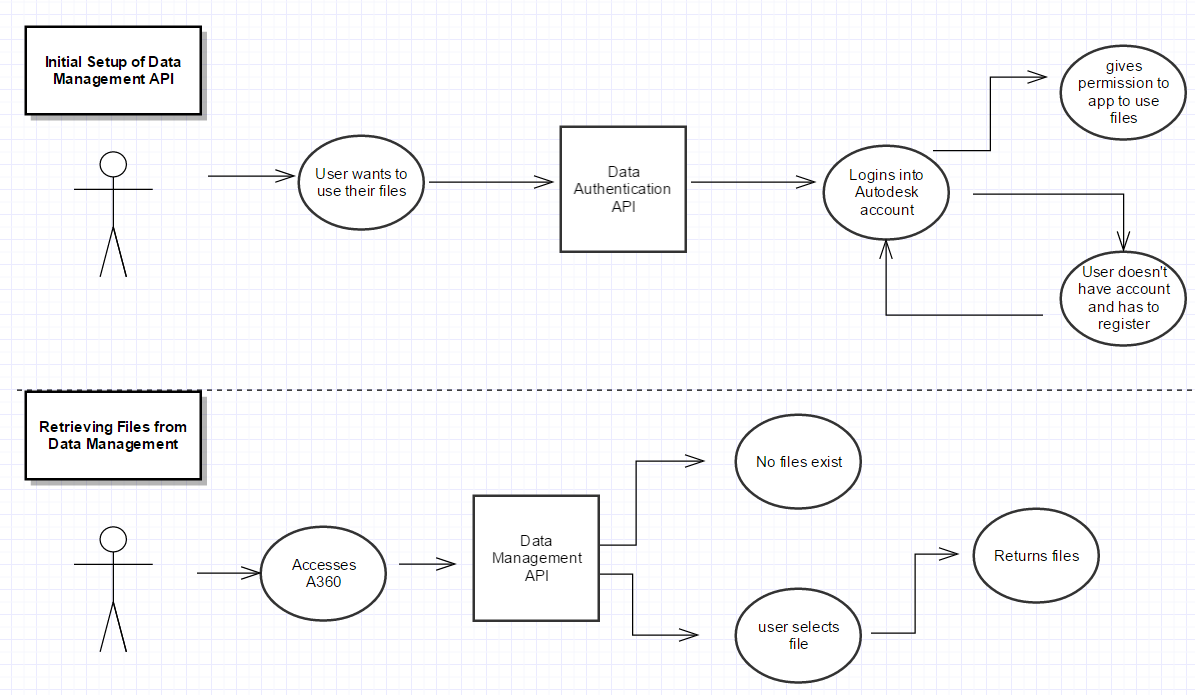
\includegraphics[scale=0.6]{DataManageUseCase.png}
	\caption{Data Management UML use case diagram}
\end{figure}
\newpage
\begin{figure}[ht]
	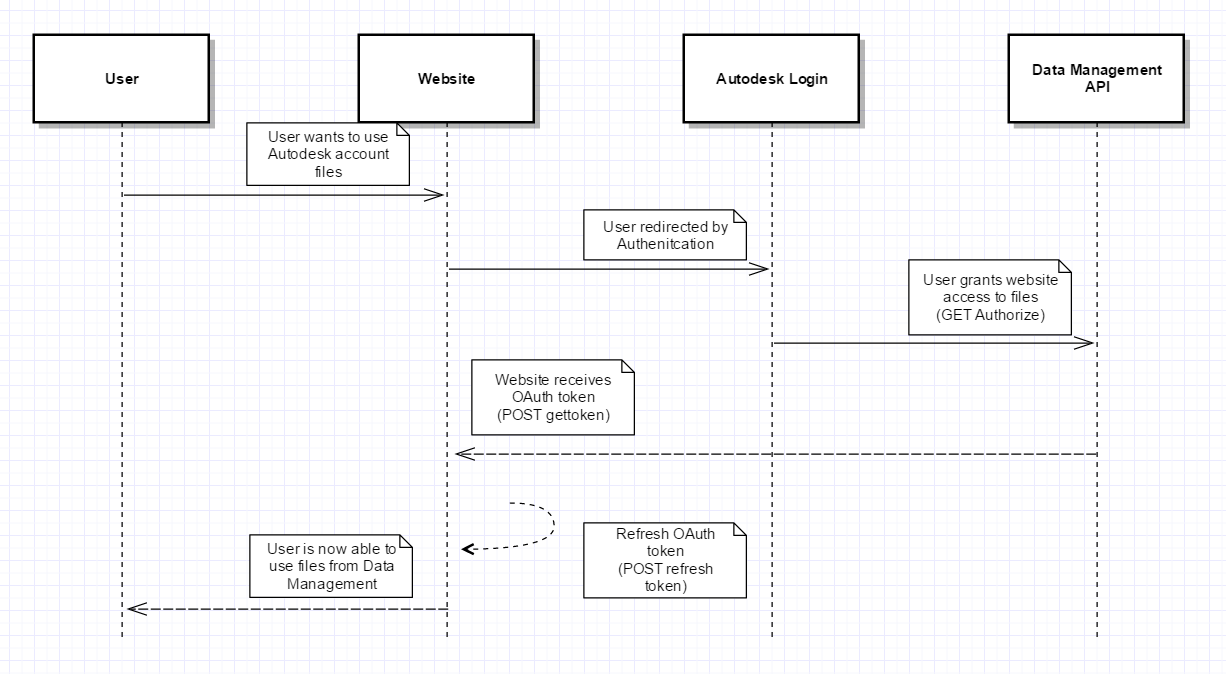
\includegraphics[scale=0.6]{Authentication3legged.png}
	\caption{3 Legged Authentication}
\end{figure}
\newpage
\begin{figure}[ht]
	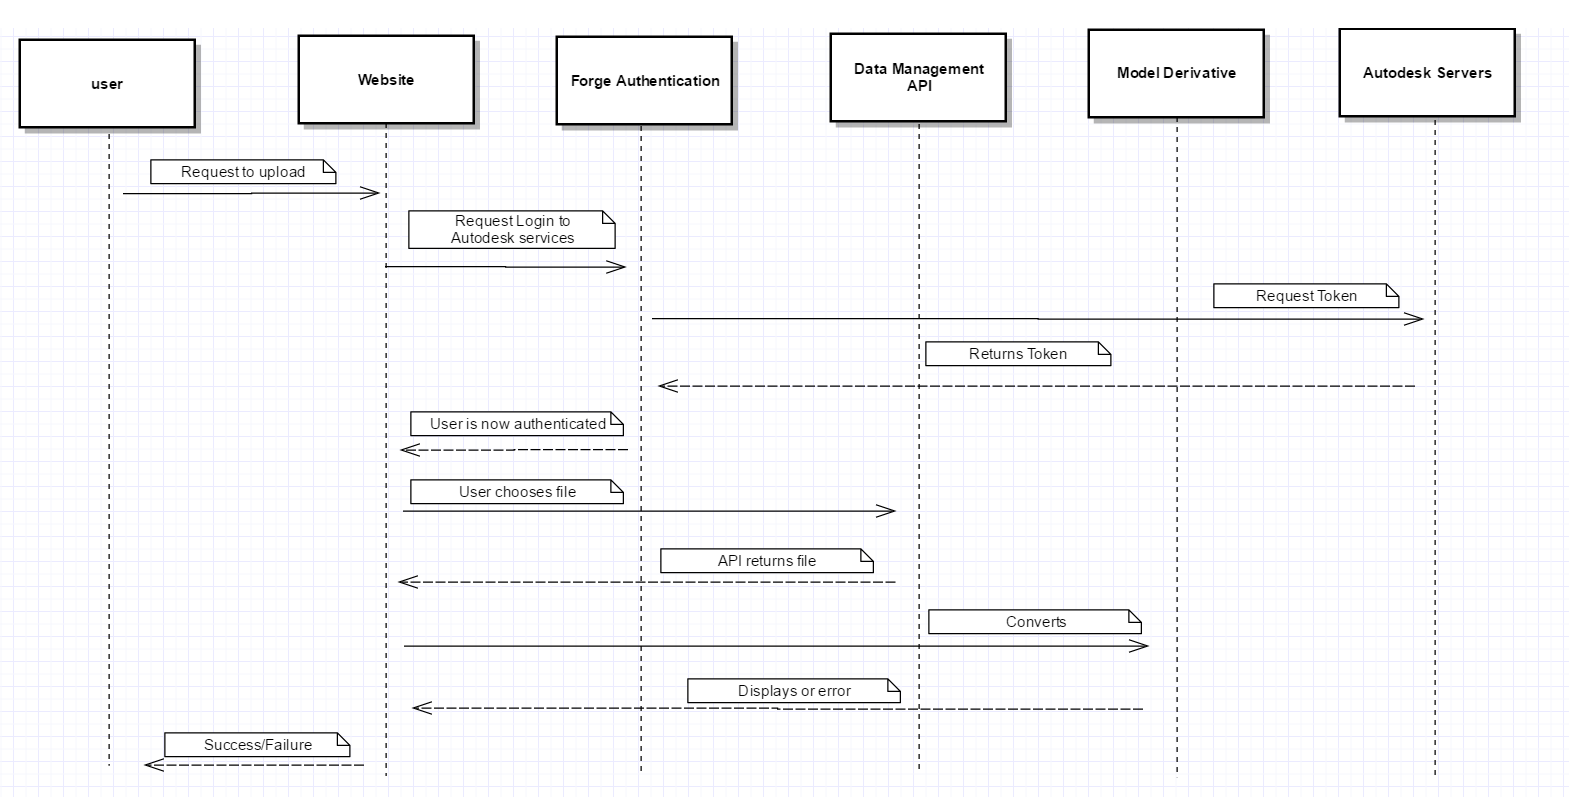
\includegraphics[scale=0.4]{nonLocalUpload.png}
	\caption{Non Local upload }
\end{figure}
\newpage
\begin{figure}[ht]
	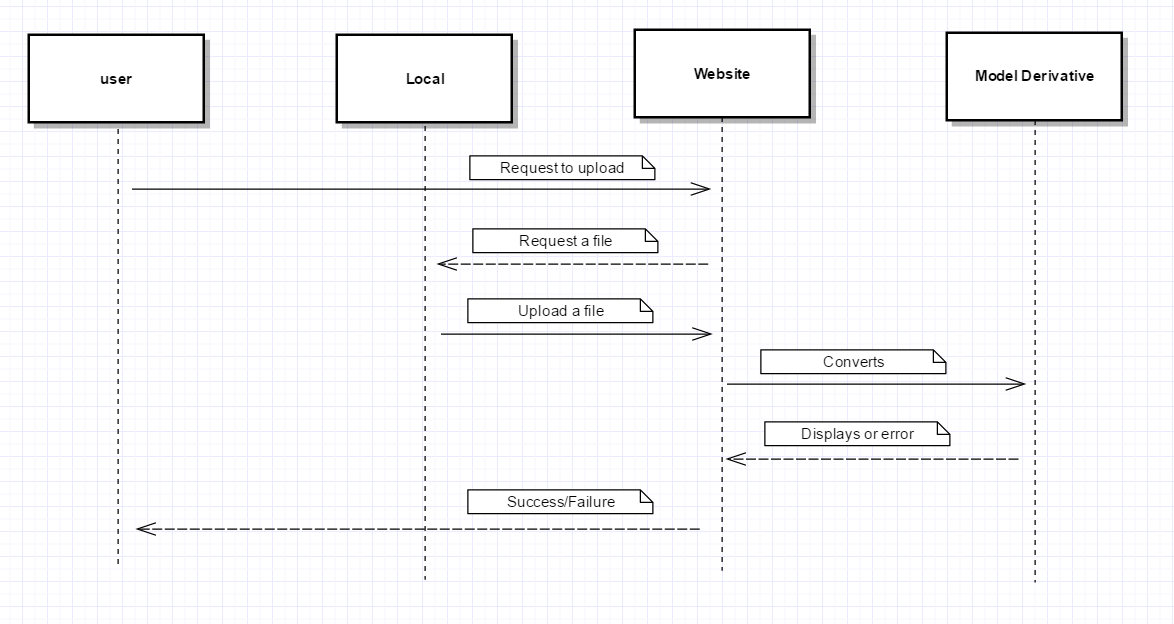
\includegraphics[scale=0.6]{localUpload.png}
	\caption{Local upload}
\end{figure}
\newpage
Our website is already up and functioning but if one desired to create the website from the ground up they would take these steps. Set-up a Heroku application. Use the server files provided within our github and connect them to the Heroku. Next sign up for a Autodesk Forge account and create an app. In this app make sure to get the client secret and ID. Change the server files to correspond to that secret and ID. In the Forge callback URL make sure to use the Heroku URL with the '/api/forge/callback/oauth' extension. Using these steps our version with the login should work after this, the user would have to setup their own bucket and and load models into it to have the models clickable on the site.\\

To run the site you need to have CAD file located on the user's local machine or the user must have some in an Autodesk account that user have access to. Then you have to upload the file to the website. Once the file is uploaded the user will then be able to interact with the object in the viewer on the website. If other people have have the link to the current session they will be able to join that session and then be able to see what the host is seeing and doing to the object in the viewer. This give the users an opportunity to have a conference about the object over the Internet. Users can also view these models in a VR environment by scanning a QR code on the website with a compatible phone and a Google cardboard headset.\\

\section{How we learned the technology}
Helpful website include: stackoverflow, github and google. We did not have anyone on campus that was a great help. But our mentors Kean and Adam who are Autodesk employees made themselves available to us. They were an immense help in getting this project done.

\section{What We Learned}
\subsection{Shawn Cross}
What technical information did you learn?

What non-technical information did you learn?

What have you learned about project work?

What have you learned about project management?

What have you learned about working in teams?

If you could do it all over, what would you do differently

\subsection{Paul Kwak}
What technical information did you learn?

How to learn, read, write and understand Javascript. As well as, setting up a server using Heroku. Debugging and adapting API as well as prewritten code.

What non-technical information did you learn?

How work as a group, organizing weekly meetings, how to function as a team as well as a communicating long distance and short distance. To delve more into this, working as a group is something thats done from a young age in school. However, most times the stakes are low, in capstone the stakes are much higher. It is considered a contract and there are potential dollars at stake for the clients. In the case of the student, time which is a valuable variable could be wasted. The penalty for failure is large number of dollars as well as an entire year of schooling. Moving on to weekly meetings, even for professionals like our client, there were many times where not all members were able to be present. The value in being able to attend each and every meeting was quite high, simply being able to attend, let alone organize a meeting is an imperative skill to have. Communication is very difficult, technology is able to keep is contact more, but also allows us to hide if need be. Many tasks can be taken care of from long distance, but the most work was always done face to face. The value in being able to decide when each is the best choice is important.

What have you learned about project work?

There are many complications, the more pieces there are the more has to be done. Even when looking to optimize work load it can take lots of time and effort to document what has been changed. For instance simply adapting a pre-built library saved us countless hours, but even so we had to spend a large amount of time to make sure it worked. On top of that, we had to fill out a large amount of documentation talking about this change. The more is added the more project work we have to do as well.

What have you learned about project management?

Having one person be a dedicated leader goes a long way. Fact of the matter is, all work is not the same. There will less in certain areas and more in others, but having a leader to delegate and split the work as best as they can manage keeps work from being wasted. It is not always on the leader though, each member always has the responsilibity of making sure they know what others and they themselves are to do.

What have you learned about working in teams?

I believe the points mentioned above answer this question well.

If you could do it all over, what would you do differently

If I were to redo the project from Fall could tell myself things, I would tell myself to take a larger initiative in leadering the project and to start work early to have more time with bugs and such. Advance working, doing things as soon as possible to account for any sort of situation ( technology problems, communication break down, etc).

\subsection{Griffin Gonslaves}
What technical information did you learn?

What non-technical information did you learn?

What have you learned about project work?

What have you learned about project management?

What have you learned about working in teams?

If you could do it all over, what would you do differently
\end{document}
